%%% ---------------------------------------------------------------------------------
%%% Vorlage Abschlussarbeit (LaTeX)
%%%
%%% V1   03/2017, Stefan Etschberger (HSA)
%%% V1.1 04/2021, rnw-hack für biblatex-run
%%% V2   05/2021, Titelblatt und Erweiterungen: Stefan Jansen (HSA)
%%% V2.1 05/2021, Trennung von R-Support und einfachem LaTeX: Phillip Heidegger (HSA)
%%% V2.2 01/2024, Anpassung an THA-Layout
%%% V3   01/2024, I18n
%%% ---------------------------------------------------------------------------------
\documentclass[
	12pt,
	a4paper %
	,
	oneside % Fuer Veröffentlichung
	,
	titlepage,
	DIV=13,
	headinclude,
	footinclude=false %
	,
	cleardoublepage=empty %
	,
	parskip=half,
]{scrreprt}

\usepackage[utf8]{inputenc}
\usepackage[T1]{fontenc}
\usepackage[hidelinks]{hyperref}
\usepackage{xcolor}
\usepackage[printonlyused]{acronym}

\usepackage[
	authorName={Lukas Konietzka},
	authorEnrolmentNo={2122553},
	authorStreet={Sebastian-Kneipp-Gasse 6A},
	authorZip={86152},
	authorCity={Augsburg},
	authorEMail={lukas.konietzka@tha.de},
	authorPhone={+49\,172-2728-376},
	authorSignaturePlace={Augsburg},
	studyProgram={Informatik},
	thesisType={Bachelorarbeit},
	thesisTitle={Automatische Segmentierung von \\ Mikro-CT-Aufnahmen zur Untersuchung \\ zahnmedizinischer Strukturen},
	studyDegree={{Bachelor of Science (B.\,Sc.)}},
	faculty={{Fakultät für \\ Informatik}},
	topicAssignment={14. November, 2024},
	submissionDate={18. März, 2025},
	%defenseDate={März 20, 2025},
	nonDisclosure={false},
	supervisor={Prof. Dr. Peter Rösch},
	supervisorDeputy={Prof. Dr. Gundolf Kiefer},
	language={de}
]{THA-Abschlussarbeit}

% Literaturdatenbank (.bib-Datei) aus Citavi o.ä.
\bibliography{Literatur_Abschlussarbeit}

\graphicspath{{Bilder/}}

\usepackage[
	format=plain,
	labelfont=bf,
	textfont=it,
	justification=raggedright,
	singlelinecheck=false
]{caption}
\DeclareCaptionLabelFormat{something}{#2.#1.}
\captionsetup[lstlisting]{labelformat=something}

\begin{document}
	% Sprachauswahl zum Umschalten innerhalb des Textes.
	% Alternativen: \thesisLanguage, ngerman, english
	\selectlanguage{\thesisLanguage}
	\pagenumbering{roman}
	\setcounter{page}{1}

	\THAtitlepage

	\let
	\cleardoublepage
	\relax

	%%% --------------------------------------------------
	%%% Kurzfassung
	%%% --------------------------------------------------
	\begin{abstract}
		\section*{Kurzfassung}
		Mikro-CT bildet eine zentrale Forschungsgrundlage der Zahnmedizin und dient als
		Basis für viele weitere Forschungen. Auch diese vorliegende Arbeit baut auf
		dieser Technologie auf und widmet sich der Entwicklung einer Erweiterung für
		3D Slicer, die die anatomische Segmentierung von Zähnen vereinfacht. Die
		anatomische Segmentierung ist ein wichtiger Prozess in der zahnmedizinischen
		Forschung, bei dem ein Mikro-CT-Bild eines Zahnes in seine anatomischen Hauptbestandteile
		unterteilt wird. Diese Segmentierung bildet die Grundlage für weiterführende
		Analysen, wie die 3D-Rekonstruktion von Zahnstrukturen oder das Training neuronaler
		Netze zur Erkennung von Karies. Der aktuelle Stand der Technik zeigt, dass bereits
		ein funktionierendes Verfahren zur anatomischen Segmentierung existiert,
		dessen Nutzung jedoch durch eine komplexe, terminal basierte Ausführung erschwert
		wird. Dies stellt insbesondere für Anwender in klinischen Praxen eine Hürde
		dar. Ziel dieser Arbeit ist es daher, eine benutzerfreundliche Lösung zu
		entwickeln, die die Funktionalität der anatomischen Segmentierung effizient in
		3D Slicer integriert und deren Anwendung erleichtert. Im Laufe der
		Entwicklung entsteht so der Tooth Analyser, der es möglich macht den Algorithmus
		der anatomischen Segmentierung mit nur wenigen Klicks über eine Benutzerschnittstelle
		zu starten und so die Benutzerfreundlichkeit erheblich zu steigern. Während
		der Entwicklung selbst entsteht nicht nur eine Software mit Funktionalität, es
		wird eine ganze Struktur beschrieben, mit der eine Verarbeitung von Mikro-CT-Bilder
		effizient, flexible und interaktiv durchgeführt werden kann. Neben dem
		Mehrwert, den die Anwendung für die praktizierenden Ärzte liefert, konnten
		auch viele Erfahrungen mit der Entwicklung in 3D Slicer gesammelt werden. So
		wird beispielsweise erläutert, wie die Plug-in-Infrastruktur der Plattform
		funktioniert und wie schließlich sichergestellt wird, das ein erstelltes Modul
		ein Softwareupdate von Slicer überlebt. Die detaillierte Evaluation des
		Tooth Analyser wird zeigen, das die geforderte Integration eines bereits existierenden
		Verfahrens in die Plattform 3D Slicer durchaus als Erfolg betrachtet werden kann.
		Jedoch wird auch sichtbar, dass das Modul in mancher Hinsicht noch einschränkend
		ist und Wünsche offen lässt.
	\end{abstract}

	%%% --------------------------------------------------
	%%% Logo ToothAnalyser
	%%% --------------------------------------------------
	\clearpage
	\vfill
	\begin{figure}
		\centering
		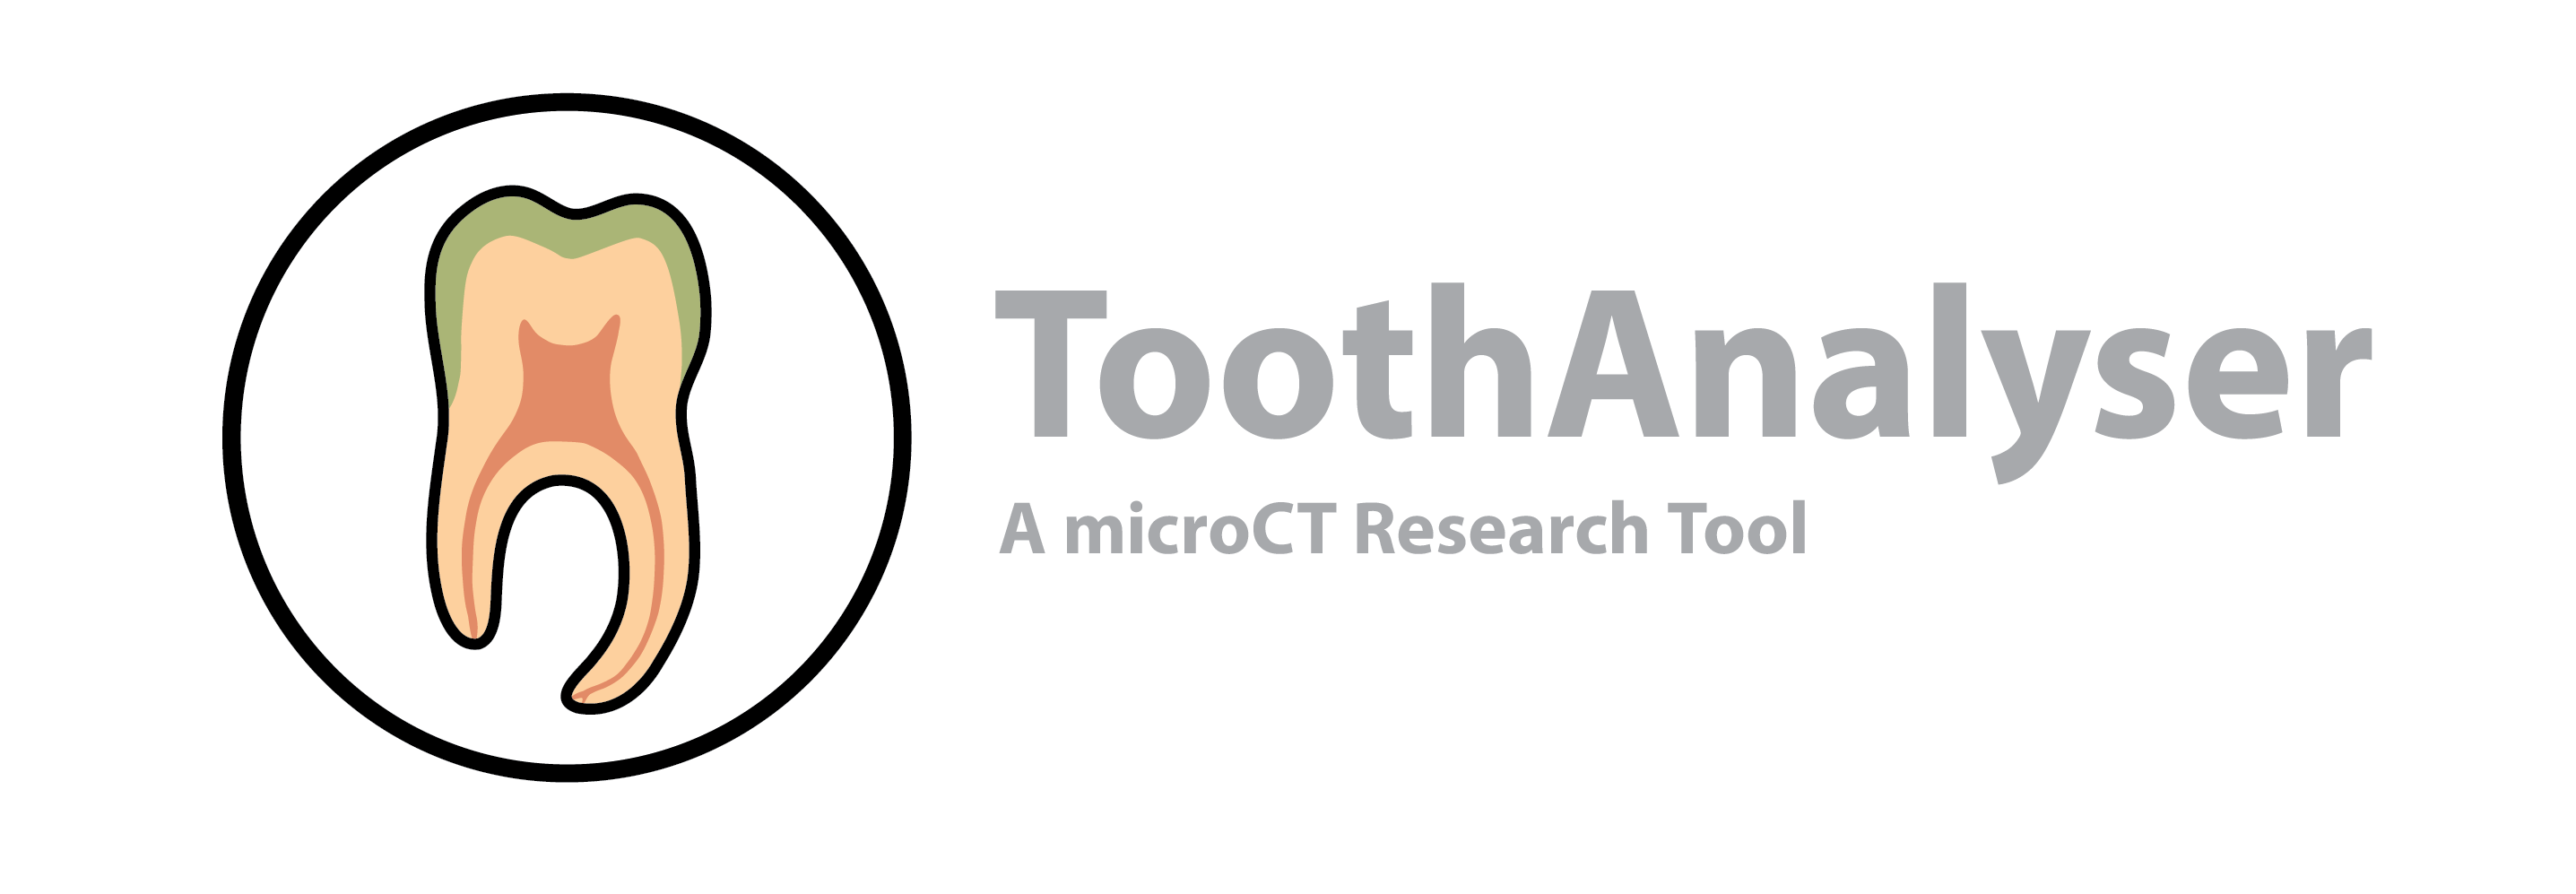
\includegraphics[width=1\textwidth]{img/SlicerToothAnalyser.png}
	\end{figure}
	\vfill
	\clearpage

	%%% --------------------------------------------------
	%%% Inhaltsverzeichnis
	%%% --------------------------------------------------
	\tableofcontents

	%%% --------------------------------------------------
	%%% Verzeichnisse
	%%% --------------------------------------------------
	\listoffigures % Abbildungsverzeichnis
	\addcontentsline{toc}{chapter}{Abbildungsverzeichnis}

	%%% --------------------------------------------------
	%%% Abkürzungsverzeichnis
	%%% --------------------------------------------------

	\chapter*{Abkürzungsverzeichnis}
	\begin{acronym}
		[ITK-SNAP, BMBF] \acro{2D}{zweidimensionalen} \acro{3D}{dreidimensonale}
		\acro{8UInt}{8 bit unsigend integer} \acro{16Int}{16 bit sigend integer}
		\acro{CLI}{Kommandozeilenschnittstelle} \acro{CT}{Computertomografie} \acro{GB}{Gigabyte}
		\acro{GUI}{Grafische Benutzerschnittstelle} \acro{Html}{Hypertext Markup Language}
		\acro{ISQ}{Industrial Scan Quality} \acro{ITK}{Insight Toolkit} \acro{ITK-SNAP}{Insight Toolkit Snake Automatic Partitioning}
		\acro{JSON}{JavaScript Object Notation} \acro{LMU}{Ludwig-Maximilians-Universität München}
		\acro{MB}{Megabyte} \acro{MRT}{Magnetresonanztomografie} \acro{MHD}{Meta Header Data}
		\acro{MRML}{Medical Reality Modeling Language} \acro{MVC}{Model View Controller}
		\acro{NIfTI}{Neuroimaging Informatics Technology Initiative} \acro{NRRD}{Nearly Raw Raster Data}
		\acro{OCT}{optische Kohärenztomografie} \acro{PyPi}{Python-Paket-Index}
		\acro{SEM}{Slicer Extension Module} \acro{SSH}{Secure Shell} \acro{THA}{Technische Hochschule Augsburg}
		\acro{UI}{Benutzerschnittstelle} \acro{UML}{Unified Modeling Language} \acro{UX}{Benutzererfahrung}
		\acro{VTK}{Visualization Toolkit} \acro{XML}{Extensible Markup Language}
		\acro{X-Ray}{Röntgenstrahlung}
	\end{acronym}
	\addcontentsline{toc}{chapter}{Abkürzungsverzeichnis}

	\renewcommand{\lstlistlistingname}{Quellcodeverzeichnis}
	\lstlistoflistings % Listings
	\addcontentsline{toc}{chapter}{Quellcodeverzeichnis}
	\listoftables % Tabellenverzeichnis
	\addcontentsline{toc}{chapter}{Tabellenverzeichnis}

	%%% --------------------------------------------------
	%%% Ab hier: Inhalt
	%%% --------------------------------------------------

	\cleardoubleoddpage
	\setcounter{page}{1}
	\pagenumbering{arabic}

	\chapter{Einleitung}
\label{chap:einleitung} Die Computertomografie (CT) hat die Medizintechnik revolutioniert
und ist bis heute eines der wichtigsten Methoden für die Bildanalyse. Sie ist
eine der führenden Erweiterungen der klassischen Röntgentechnik. Für die Entwicklung
dieser Technologie wurden Godfrey Newbold Hounsfield und Allan McLeod Cormack im
Jahre 1979 mit dem Nobelpreis für Medizin ausgezeichnet \citep[Seite12]{handels2000}.

\begin{minipage}{0.40\textwidth}
	Die Computertomografie wird in den verschiedensten Bereichen und im wahrsten Sinne
	des Wortes von Kopf bis Fuß eingesetzt. So kommt es, dass auch im Dentalbereich
	CT Aufnahmen von größter Wichtigkeit sind. Abbildung
	\ref{fig:ct_aufnahme_eines_zahns} zeigt eine solche CT-Aufnahem. Eine konkrete
	Anwendung in diesem Kontext ist die Zahnkaries Forschung der Poliklinik für Zahnerhaltung
	und Parodontologie des LMU- Klinikums München.
\end{minipage}
\hfill
\begin{minipage}{0.50\textwidth}
	\centering
	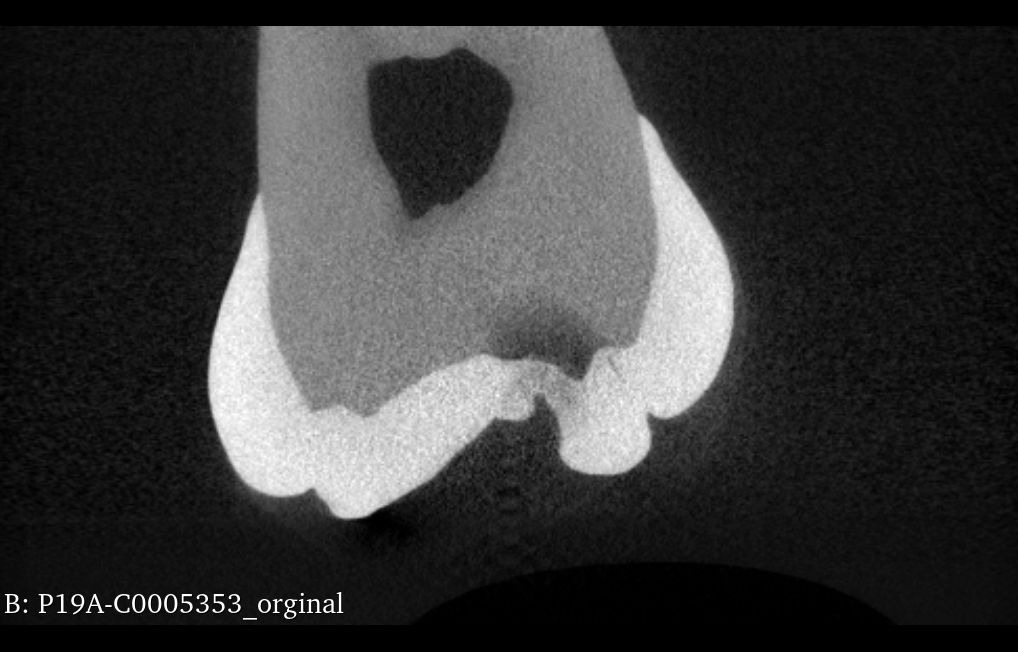
\includegraphics[scale=0.2, width=\textwidth]{img/micro_ct_orginal.jpg}
	\captionof{figure}{CT-Aufnahme eines Zahns \\ Quelle \citep{poliklinikLMU}} \label{fig:ct_aufnahme_eines_zahns}
\end{minipage}

Die vorliegende Arbeit soll genau diese Forschung unterstützen. In welchem Umfang
und zu welchem Grund ist in den folgenden Abschnitten beschrieben.
% ---------------------------------------------------------------------------------------

\section{Ziel der Arbeit}
\label{sec:ziel_der_arbeit} Diese Arbeit beschreibt eine Technik, mit der
dreidimensionale Micro-CT Bilder zur Untersuchung zahnmedizinischen Strukturen
automatisch mittels der Software \textit{3D Slicer} segmentiert und analysiert werden
können. Die algorithmische Formulierung einer konkreten Segmentierung ist
bereits vorhanden und prototypisch implementiert. Dieser Algorithmus muss jedoch
umständlich über ein Kommando im Terminal ausgeführt werden, was die
Benutzerfreundlichkeit deutlich beeinträchtigt. Ziel dieser Arbeit ist es nun das
bereits implementiert Verfahren automatisiert über ein interaktives User Interface
(UI) zur Verfügung zu stellen. Dabei soll auf etablierte und vertraute Lösungen
zurückgegriffen werden.

Es stellt sich nun die Frage, zu welchem Zweck eine automatische und interaktive
Segmentierung überhaupt notwendig ist. Für die Zahnklinik an der LMU in München
gibt es hierfür viele Gründe. Über den wichtigsten gibt das nächste Kapitel Aufschluss.
% ---------------------------------------------------------------------------------------

\section{Relevanz der Arbeit}
\label{sec:relevanz_der_arbeit} Der wohl relevanteste Punkt dieser Arbeit ist,
dass Ärzte reine Anwender und keine Entwickler von Software sind. Darüber hinaus
verfolgt die Parodontologie der LMU in München einen sehr interessanten Forschungsansatz,
welche eine Segmentbetrachtung der CTs unumgänglich macht.

Über viele Jahre hinweg wurden in der Zahnklinik sehr viel Bilddaten von Zähnen
gesammelt, die aufgrund von Zahnkaries entfernt wurden. Hierbei wurden Aufnahmen
der unterschiedlichsten Arten gemacht. Darunter fallen zum Beispiel einfache Bilddateien,
Infrarotbilder und die für diese Arbeit so relevanten dreidimensionalen (3D)
Micro-CT Aufnahmen. Dieser große Schatz an Bildmaterial soll verwendet werden,
um in ferner Zukunft ein neuronales Netzwerk zu trainieren, welches statistische
Aussagen über das Verhalten von Karies treffen kann. Jedoch gibt es hier ein
Problem, bei dem das Ergebnis dieser Arbeit Unterstützen kann. Karies auf CT-Bildern
zu lokalisieren ist nicht trivial. Er ist ohne weitere Bearbeitung des Bildes nur
sehr schwer auf eine Stelle einzugrenzen. So kommt es vor, dass drei verschiedene
Ärzte auf dem selben Micro-CT Bild drei unterschiedliche Stellen mit Karies identifizieren.
Eine Segmentierung des dreidimensionalen CTs kann hier Wunder wirken lassen. Durch
die Aufteilung des Micro-CTs in seine zwei Zahnhauptsubstanzen, kann in das
innere der Zähne geblickt werden, was die Lokalisierung kariöser Stellen deutlich
vereinfacht.

Mit dieser klaren und einduetigen identifizierung von Karies, sind die
Ergebnisse, die ein neuronales Netzer generieren würde viel genauer und brauchbarer.
Konkret wird mit einer automatischen Segmentierung ein \textit{Ground Trueth} gewonnen,
der eine eindeutige Basiswahrheit liefert. Hierbe sei gesagt das diese Anwendung
nur ein von vielen Möglichkeiten ist. Konkrete Daten über die Ausbreitung einer
Krankheit im Menschlichen Körper zu besitzten kann in den verschiedensten Fällen
und Institutionen von größtem Nutzen sein. So zeigen es auch \citet{de20083d} in
ihrem Paper.

Anhand dieser Argumente wird deutlich, dass eine automatische Segmentierung durchaus
einen mehrwert für Ärzte bilden kann. Für eine automatische Segmentierung von
Micro-CT Bildern gibt es einige Softwarelösungen am Markt, die alle eine gut optionen
sind. Aus diesem Gurnd wird soll folgenden Kapitel ein mögliches Framework
diskoutiert werden.
% ---------------------------------------------------------------------------------------

\section{Fokus der Arbeit}
\label{sec:fokus_der-arbeit} Dieser Arbeit setzt den Fokus auf die Open Sorce
Plattform \textit{3D Slicer}, da diese ohnehin bereits eine breite Anwendung in
der Zahnklinik in München findet. Durch die Modul und Plugin Infrastruktur dieser
Plattform kann die Softwar auch anderen Institutionen bereitgestellt werden.
Hierzu muss diese einfach als \textit{3D Slicer Extetion} bereitgestellt werden.
\textit{3DSlicer} bietet einen Extension Manager, der ähnlich wie ein App Store
betrachtet werden kann. So bleibt die vorerst konkret entwickelte Software nicht
nur einer Einrichtung vorbehalten. Die Optimierung des bereits bestehenden, prototypischen
Verfahrens wird nicht thematisiert.

Mit diesem Umfang, der Motiavtion und dem gesetzten Fokus, ergibt sich für dies Arbeit
eine konkrete Struktur, die einen hohen detailgrad aufweisen wird. Um einen Überblich
zu gewähren, sei diese Struktr hier kurz eräutert.
% ---------------------------------------------------------------------------------------

\section{Aufbau der Arbeit}
\label{sec:aufbau_der_arbeit} Die Arbeit ist in sieben Kapitel unterteilt. Nach der
Einführung in Kapitel \ref{chap:einleitung}, in der die Relevanz und der Fokus
beschrieben werden, werden in Kapitel \ref{chap:theoretische_grundlagen} die theoretischen
und technischen Grundlagen behandelt, welche zum Verstehen der Ergebnisse
essenziell sind. Als Ergebnis der theoretischen Grundlagen bildet das Kapitel \ref{chap:fragestellung}
eine konkrete Forschungsfrage. Während sich Kapitel \ref{chap:methodik} darum
kümmert mit welchen Methodiken und Lösungsansätzen an die Forschungsfrage
herrangegangen wird, erläutert das Kapitel \ref{chap:ergebnisse} was die konkreten
Ergebnisse der Arbeit sind. In Kapitel \ref{chap:diskussion} erfolgt eine
kritische Diskussio der Resultate einschließich möglicher Limitationen. Das Abschließende
Kapitel\ref{chap:schlussfolgerung} fasst die wichtigsten Erkenntnisse zusammen
und gibt einen Ausblick auf zukünftige Forschungsfragen.

Die theoretischen Grundlagen die wie beschrieben direkt nach der Einleitung
folgen, sind zentral für das Versetehen der Fragestellung und der später folgenden
Ergebnisse der Arbeit.
% ---------------------------------------------------------------------------------------
	\chapter{Anatomische Segmentierung}
\label{chap:theoretische_grundlagen} Die anatomische Segmentierung ist ein bestehendes
Verfahren, das bereits von der Klinik an der LMU eingesetzt wird, um segmentierte
Daten aus Mikro-\ac{CT}-Bildern gezielt zu gewinnen. Einen wichtigen Meilenstein
hierfür liefert Hofmann. Im Rahmen einer Bachelorarbeit an der Hochschule für
angewandte Wissenschaften in Augsburg unterstützte Herr Hofmann die
Kariesklassifizierung auf den Zahnkronen-\ac{CT}-Aufnahmen. Hierzu entwickelte
er ein Verfahren, das auf Basis von Schwellwertverfahren die Zahnsubstanzen Schmelz
und Dentin aus dem Originalbild herauslöst. Dabei wird die anatomische
Segmentierung als der Prozess verstanden, bei dem diese Gewebetypen gezielt voneinander
getrennt und visuell sowie rechnerisch unterscheidbar gemacht werden.

\begin{minipage}{0.40\textwidth}
	Durch die Segmentbetrachtung der beiden Gewebesubstanzen Schmelz und Dentin konnte
	\citet[S.~41]{hoffmann2020} eine gute Hilfe für die Befundung kariöse Stellen
	liefern. Ein Ergebnis aus der Arbeit von Hofmann sei in Abbildung \ref{fig:ergebnis_hoffmann}
	gezeigt. Hierfür entwickelte Hofmann ein prototypisches Verfahren innerhalb
	eines IPython Notebooks, mit dem es gelang ca. 250 Datensätze der Klinik
	automatisch aufzubereiten.
\end{minipage}
\hfill
\begin{minipage}{0.50\textwidth}
	\centering
	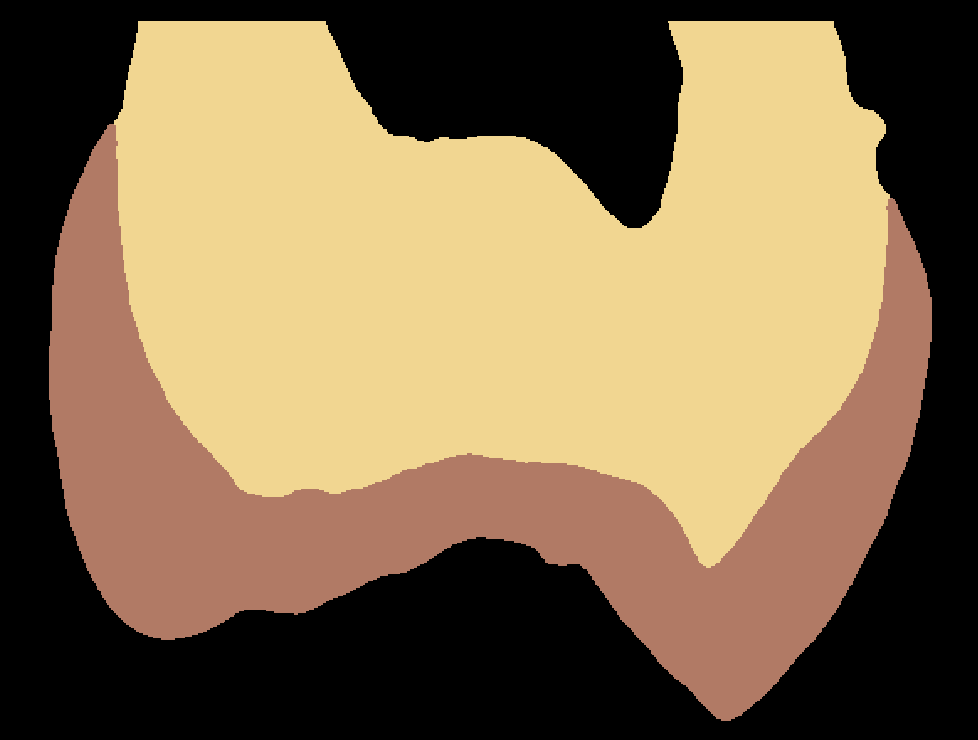
\includegraphics[width=0.7\textwidth]{img/ergebnis_hoffmann_2.jpg}
	\captionof{figure}{Reproduziertes Ergebnis der anatomischen Segmentierung} \label{fig:ergebnis_hoffmann}
\end{minipage}

Neben der Erstellung von segmentierten Daten stellt das Verfahren noch
sogenannte mediale Flächen zur Verfügung. Diese sind insbesondere für die Klassifizierung
von Karies notwendig. \citet[S.~42]{hoffmann2020} erklärt, das sich bei einer
Überlagerung der medialen Flächen auf das Originale Bild auf einem Blick
erkennen lässt, ob die vorhandene Karies in diesen Schichten weiter als die Hälfte
fortgeschritten ist. Für die Erstellung der medial Flächen sind die segmentierte
Daten eines Zahnes zwingend erforderlich. Die Berechnung der medial Flächen erfolgte
auf den Segmenten mithilfe einer Distanztransformation und anschließender Kantenfindung
\citep[vgl.][S.~42]{hoffmann2020}.

Die anatomische Segmentierung eines Zahnes – einschließlich der medialen Flächen
– erfolgt in mehreren algorithmischen Schritten, die in einer klar strukturierten
Pipeline ablaufen. Abbildung \ref{fig:anatomische_segmentierung} veranschaulicht
den groben Ablauf des Verfahrens, wobei kleinere Zwischenschritte ausgeklammert sind.
Der Prozess beginnt oben links und endet mit der Generierung der medialen
Flächen in der unteren rechten Ecke.

\begin{figure}[h]
	\centering
	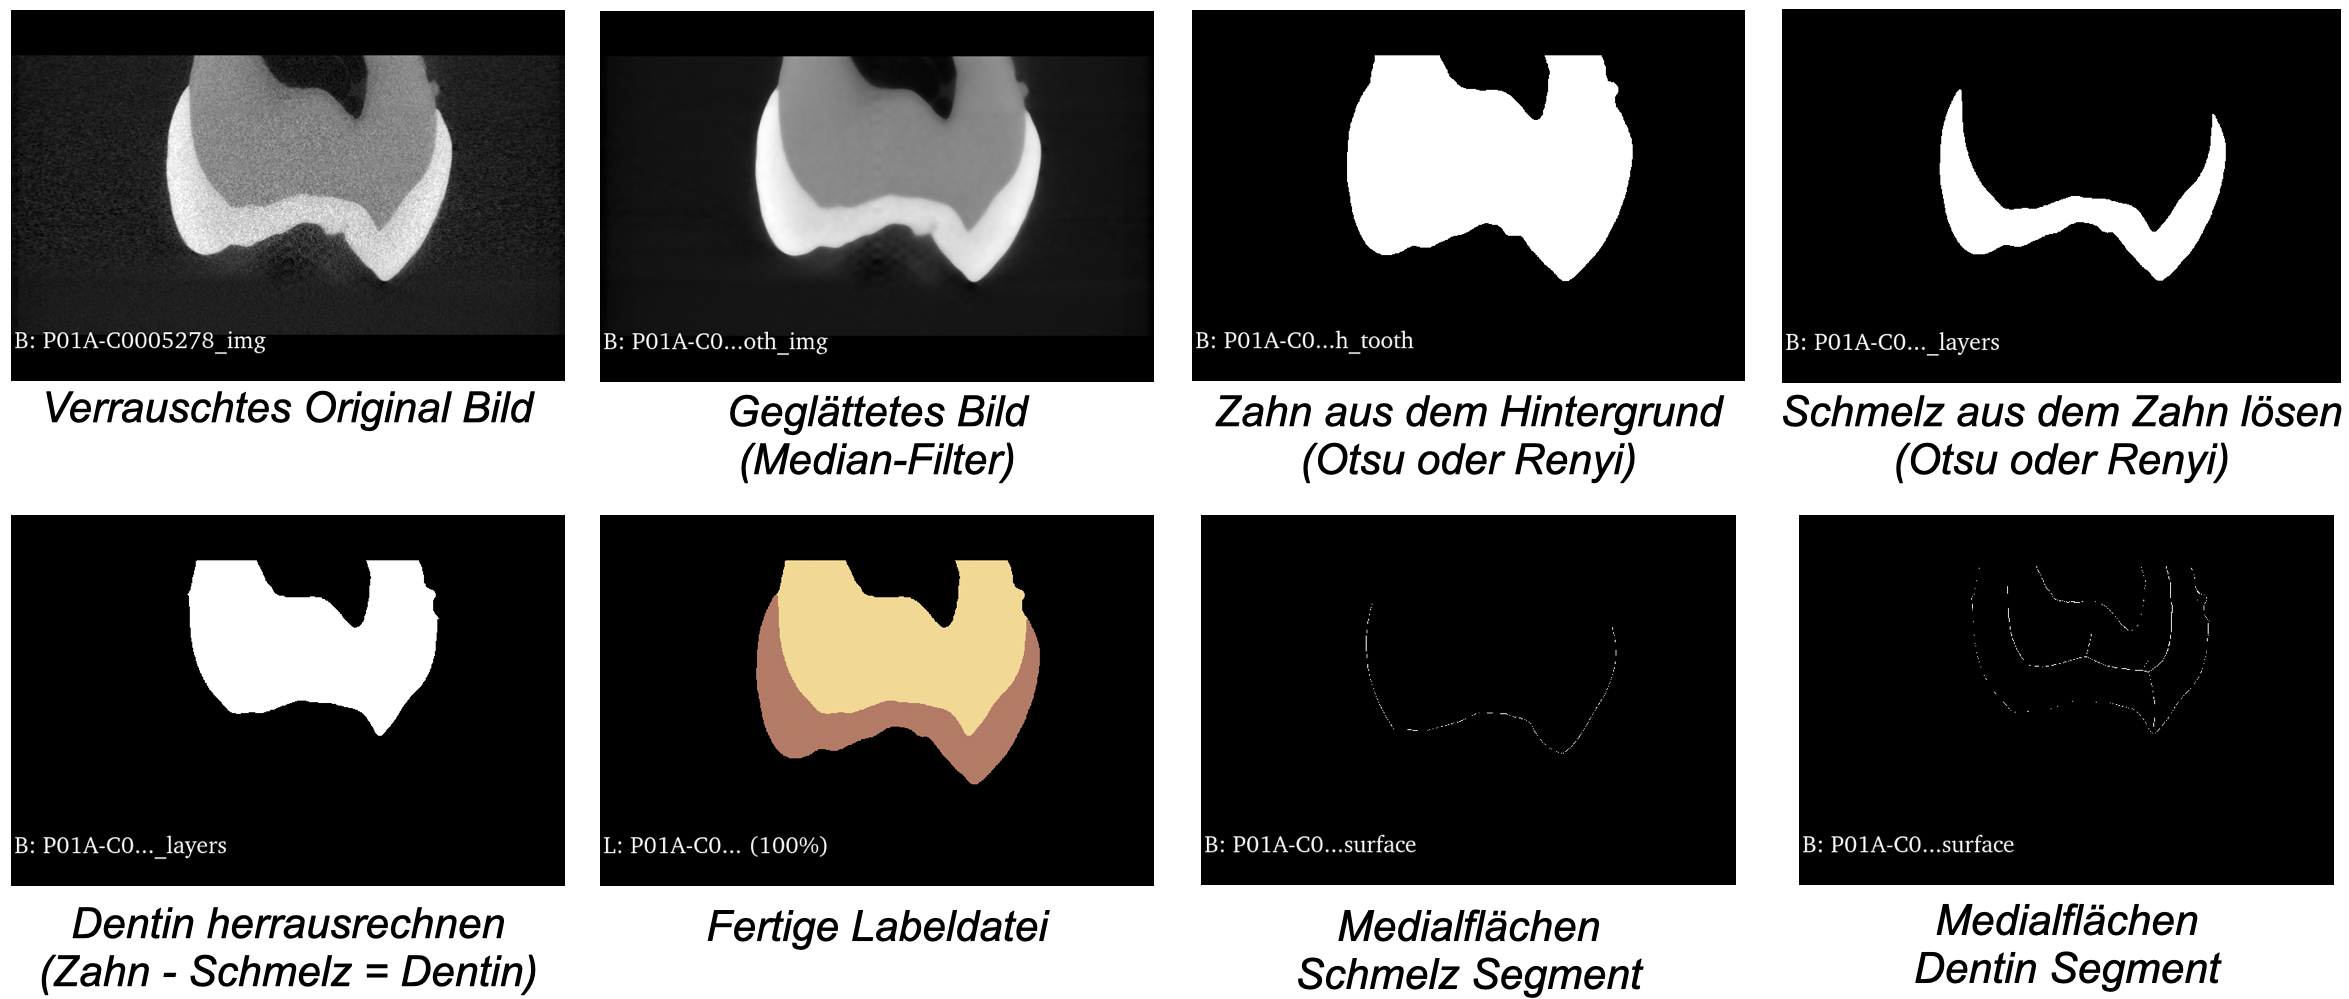
\includegraphics[width=1\textwidth]{img/anatomischeSegmentierung.png}
	\caption{Algorithmische Formulierung der anatomischen Segmentierung nach
	\citet{hoffmann2020} (von links oben nach rechts unten)}
	\label{fig:anatomische_segmentierung}
\end{figure}

Wie \citet[S.~55]{hoffmann2020} beschreibt, kann dieses Verfahren bis zu einem gewissen
Fortschritt von Karies angewendet werden. Da Karies im Laufe der Zeit zur
Zersetzung des Zahns führt, entstehen dunkle Stellen im Schmelzbereich, die die
zusammenhängenden Grauwerte im Bild stören und somit die Segmentierung
erschweren. Eine weitere Herausforderung liegt in der Art der Bilddaten, für die
das Verfahren ursprünglich entwickelt wurde. Es basiert auf \ac{ISQ}-Bildern, die
im \ac{16Int}-Format vorliegen.

Die einzelnen Schritte in Abbildung \ref{fig:anatomische_segmentierung}
verdeutlichen, dass die Segmentierung stets einem spezifischen Muster folgt und das
Verfahren primär zwischen Dentin und Schmelz unterscheidet. Die Pulpa wird wie
bereits beschrieben in diesem Verfahren nicht berücksichtigt. Zudem wird ersichtlich,
dass sowohl Filter als auch Segmentierungstechniken essenziell für eine präzise
Trennung der Strukturen sind. Um ein besseres Verständnis für diesen Prozess zu gewinnen,
führt das folgende Kapitel in die anatomischen Strukturen eines Zahns ein und
zeigt, wie diese auf Mikro-\ac{CT}-Aufnahmen erkennbar sind. Dabei werden die grundlegenden
Techniken der Bildgewinnung und -bearbeitung näher erläutert.

\pagebreak
% ---------------------------------------------------------------------------------------

\section{Anatomische Zahnstrukturen in Mikro-CT-Bildern}
\label{sec:domänenspezifisch} Um nachvollziehen zu können, wie eine \ac{CT}-Aufnahme
technisch segmentiert und in ihre einzelnen Bestandteile zerlegt werden kann,
ist es zunächst essenziell, die anatomische Struktur des Zahns genau zu verstehen.
Dazu gehören die unterschiedlichen Gewebeschichten wie Zahnschmelz, Dentin und die
Pulpa, die sich nicht nur in ihrer physikalischen Zusammensetzung, sondern auch in
ihrer radiologischen Darstellung innerhalb der \ac{CT}-Bilder unterscheiden. Erst
mit diesem grundlegenden Verständnis lassen sich Methoden zur \ac{3D}-Bildbearbeitung
ableiten.

\begin{minipage}{0.40\textwidth}
	Die Abbildung \ref{fig:aufbau_eines_zahnes} zeigt den groben Aufbau eines Zahnes
	nach \citet[S.~17]{lehmann2012Zahnheilkunde}. Zu sehen ist, dass das Denit
	oder auch Zahnbein genannt den Großteil eines Zahnes einnimmt. Im Bereich der Zahnkrone
	wird das Dentin von Zahnschmelz überzogen. Der Zahnschmelz ragt in die
	Mundhöhle und ist nach \citet[S.~41]{lehmann2012Zahnheilkunde} das härteste Material
	im menschlichen Körper. In der Mitte des Zahnes befindet sich Weichgewebe, das
	als Pulpa bezeichnet wird vgl. \citep[vgl.][S.~15]{lehmann2012Zahnheilkunde}.
	Für die anatomische Segmentierung von Zahn-\ac{CT}-Aufnahmen spielen insbesondere
	die drei Hauptbestandteile des Zahns – Schmelz, Dentin und Pulpa – eine
	entscheidende Rolle.
\end{minipage}
\hfill
\begin{minipage}{0.50\textwidth}
	\centering
	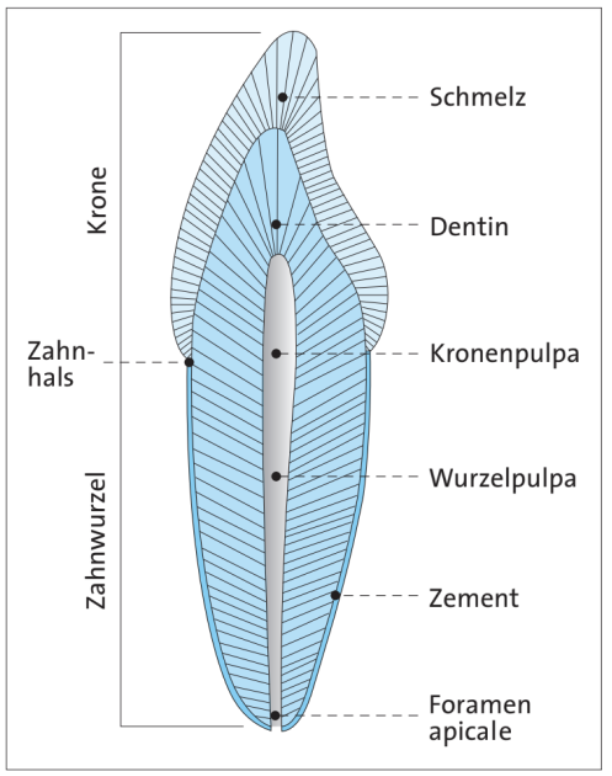
\includegraphics[scale=0.50]{img/aufbau_eines_zahns.jpg}
	\captionof{figure}{Aufbau eines ganzen Zahnes nach \citet[S.~15]{lehmann2012Zahnheilkunde}}
	\label{fig:aufbau_eines_zahnes}
\end{minipage}

Diese Gewebearten weisen unterschiedliche Strukturen auf, die sich in den
verschiedenen Graustufen auf einem Mikro-\ac{CT}-Bild widerspiegeln. Die Pulpa, das
innere Weichgewebe des Zahns, unterscheidet sich dabei nur geringfügig vom
Hintergrund, da sie als einzige der drei Hauptstrukturen nur sehr wenig Röntgenstrahlen
absorbiert. Aufgrund dieser geringen Sichtbarkeit spielt die Pulpa in dieser
Arbeit eine untergeordnete Rolle und wird nicht in das Segmentierungsverfahren
einbezogen. Geht man von innen nach außen, folgt auf die Pulpa das Dentin, das auch
als Zahnbein bezeichnet wird. Laut \citet[S.~41]{lehmann2012Zahnheilkunde} handelt
es sich dabei um eine Hartsubstanz, die den Zahn im Kieferknochen hält. Aufgrund
seiner Dichte ist das Dentin in \ac{CT}-Aufnahmen bereits deutlich erkennbar. Die
äußerste Schicht des Zahns bildet der Zahnschmelz. Dieser stellt die härteste
Substanz im menschlichen Körper dar und erscheint auf den \ac{CT}-Bildern besonders
hell. Seine hohe Dichte sorgt für eine klare Abgrenzung zu den darunterliegenden
Schichten, was ihn zu einem wichtigen Orientierungspunkt für die Segmentierung macht
\citep[vgl.][S.~41]{lehmann2012Zahnheilkunde}. Mit der folgenden Abbildung \ref{fig:pulpa_dentin_schmelz}
werden die verschiedenen Gewebearten in einem Zahn den entsprechenden Graustufen
zugeordnet.

\begin{figure}[h]
	\centering
	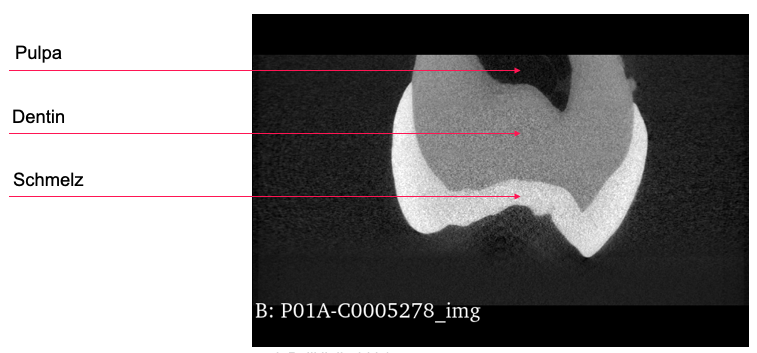
\includegraphics[width=0.9\textwidth]{img/dentin_schmelz_pulpa.png}
	\caption{Darstellung von Pulpa, Dentin und Schmelz auf einem Zahnkronen-CT nach
	\citet{heck2024}}
	\label{fig:pulpa_dentin_schmelz}
\end{figure}

Zu Beachten ist hier, dass es sich bei der in Abbildung \ref{fig:pulpa_dentin_schmelz}
gezeigten \ac{CT}-Aufnahme um eine Zahnkrone handelt und nicht um den ganzen
Zahn. Zu sehen ist auch der fast identische Grauwert zwischen dem Hintergrund und
der Pulpa.

Mit diesem Wissen über die Anatomie eines Zahnes und die Zusammensetzung auf einem
Mikro-\ac{CT}, kann nun ein Schritt weiter gegangen werden, indem der Fokus auf
die \ac{CT}-Bilder gerichtet wird. Das folgende Kapitel bietet daher einen
Überblick über die Erstellung von Röntgenaufnahmen sowie die Berechnung einer
Mikro-\ac{CT}-Aufnahme. Durch die Bildgewinnung wir auch klar, mit welcher hohen
Auflösung gearbeitet wird und warum dies auch zu Hindernissen führt.
% ---------------------------------------------------------------------------------------

\section{Erstellung von Mikro-CT-Bildern}
\label{sec:technologisch} Die Erzeugung dreidimensionaler Bilddaten ist ein essenzieller
Bestandteil der modernen medizinischen Bildgebung und kann auf verschiedene Weise
erfolgen. Je nach Anwendungsgebiet kommen unterschiedliche Verfahren zum Einsatz,
darunter \ac{MRT}, \ac{OCT} und insbesondere die Computertomografie \citep[vgl.][S.~14]{handels2000}.
Eine spezielle Variante der Computertomografie ist das Mikro-\ac{CT}, das durch
seine kleinere Ausführung in der zahnmedizinischen Forschung und Diagnostik eine
zentrale Rolle spielt. Auch die Handhabung dieser erstellten Daten ist ein wichtiger
Bestandteil der Forschung.
% ---------------------------------------------------------------------------------------

\subsection{Computertomografie}
\label{subsec:computertomografie} Die Erfindung der Computertomografie (\ac{CT})
war ein Quantensprung in der Geschichte der Medizin. Sie ist aus heutigen Diagnosen
nicht mehr wegzudenken. Ein Mikro-\ac{CT}-Bild ist laut \citet[S.~1]{baird2017}
ein Menge hochauflösender Bilder, die wie ein Stapel zusammengelegt werden.
Vereinfacht gesagt, werden so \ac{2D} Bilder zu einem \ac{3D}-\ac{CT}
zusammengesetzt. Der Aspekt Mikro deutet dabei darauf hin, dass es eine
miniaturisierte Ausführung eines üblichen Kegelstrahl-\ac{CT}s ist, so \citet[S.~340]{buzug2011}.
Eine andere Definition erläutert \citet[S.~49]{lehmann2013bildverarbeitung}. Er beschreibt
die Computertomografie als Projektionen einzelner Ebenen im Untersuchungsobjekt.
Die Abbildung \ref{fig:spectrum} soll diesen Vorgang genauer beschreiben.

\begin{figure}[h]
	\centering
	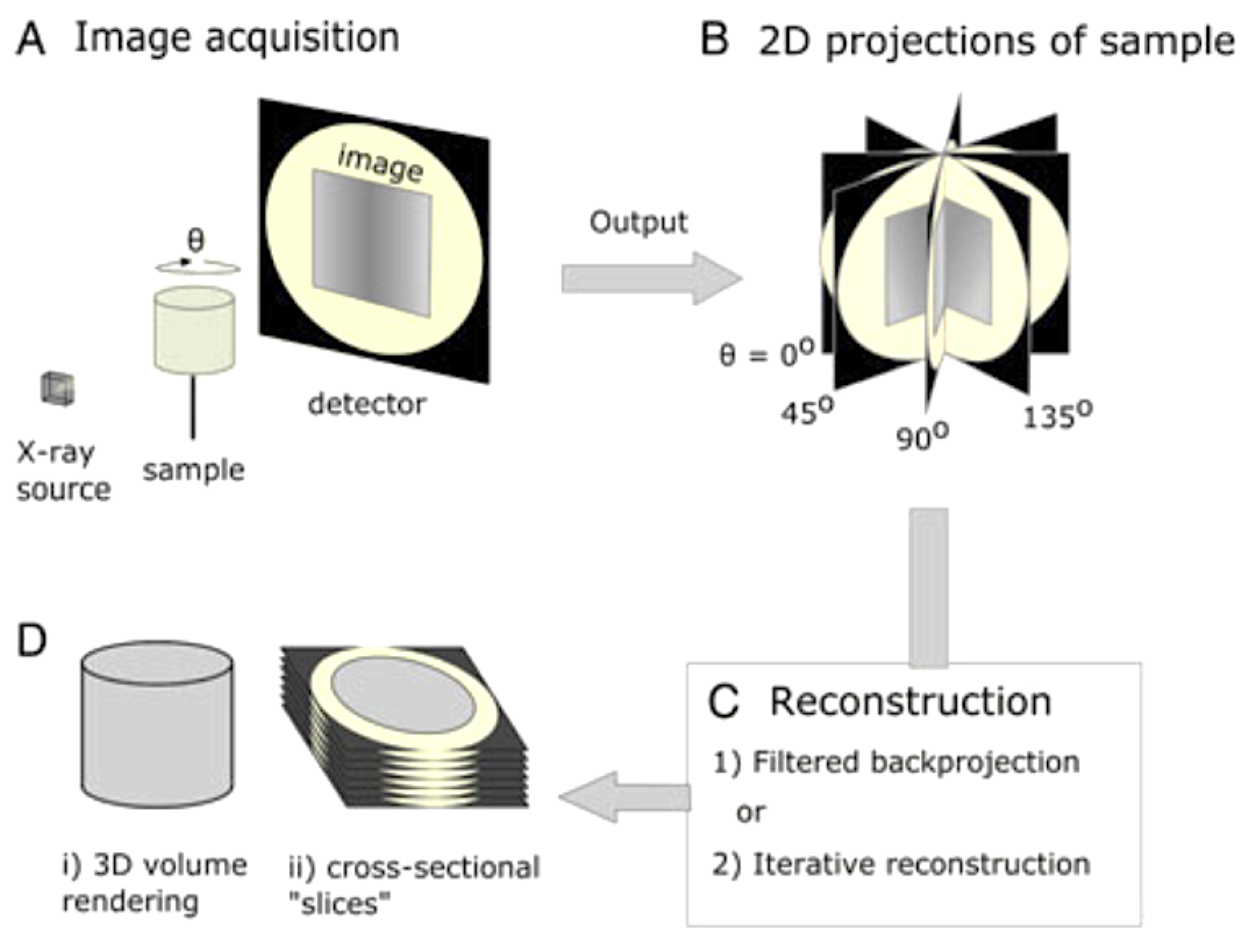
\includegraphics[width=0.6\textwidth]{img/Funktion_CT.png}
	\caption{Funktionsweise eines Mikro-CT nach \citet[S.~16]{pult2021}}
	\label{fig:spectrum}
\end{figure}

Die Technologie, mit der diese Bilder aufgenommen werden, ist unter der Röntgentechnik
oder auch \ac{X-Ray} bekannt. Die Röntgenstrahlung ist eine Form der elektromagnetischen
Strahlung, ähnlich wie das sichtbare Licht, so das \citet[K.~1]{nib2024}. Anders
als das Licht haben die Röntgenstrahlen eine viel höhere Energie. Das führt dazu,
dass man mit dieser elektromagnetischen Strahlung viele Objekte durchdringt werden
können. So auch Gewebeteile eines Zahnes \citep[vgl.][K.~1]{nib2024}. Mit der
Steigerung der Atomzahl in einem Material, also der Dichte, nimmt auch die
Absorption eines Materials zu, sodass es leicht ist, verschiedene Materialien in
einer \ac{CT}-Aufnahme zu unterscheiden \citep[vgl.][K.~1]{nib2024}. Um nun mittels
der Röntgenstrahlen und den einzelnen \ac{2D} Projektionen ein \ac{3D}-Micro-\ac{CT}
zu erstellen, werden 2D-Röntgenaufnahmen eines Objektes aus verschiedenen Winkeln
geschossen und in einem weiteren Schritt dann zu einem \ac{3D}-Modell
rekonstruiert. Das Ergebnis einer solchen Rekonstruktion ist dann eine Art Papierstapel.
Dieser besteht aus vielen 2D-Bilder, die aufgrund der Stapelung zu einem \ac{3D}-Bild
werden.

Für die Erzeugung dieser Bilder bedarf spezieller Geräte, im Falle der Zahnklinik
an der \ac{LMU} handelt es sich um ein Mikro-\ac{CT}-Gerät der Firma \citet{scanco2024}.
Dieses Gerät erstellt Aufnahmen mittels Röntgenstrahlung und generiert mithilfe der
Computertomografie ein dreidimensionales Bild, welches im Format \ac{ISQ} abgelegt
wird. Das folgende Kapitel zeigt, dass Mikro-\ac{CT}-Bilder mit dem Typ \ac{ISQ}
zwar eine hohe Detailgenauigkeit bieten, jedoch auch einen erheblichen
Speicherbedarf mit sich bringen.
% ---------------------------------------------------------------------------------------

\subsection{Datenformate}
\label{subsec:datensätze} Die rohen Datensätze, welche direkt aus dem Mikro-\ac{CT}-Gerät
kommen, haben nach \citet{scanco2024} das Format \ac{ISQ}. Dieses Format fällt
speziell auf die Geräte der Firma SCANCO zurück. Wie das vorherige Kapitel \ref{subsec:computertomografie}
bereits eingeführt hat, ist dieser Dateityp für eine weitere Bearbeitung nur
bedingt geeignet. Unter anderem wegen ihrer Größe. \citet[S.~118-119]{RoeschKunzelmann2018}
haben ein Paket entwickelt, mit dem sich gu zeigen lässt, wie sich diese großen Bilder
zusammensetzten. Hierfür konvertiert das Paket ein \ac{ISQ}-Bild in ein \ac{MHD}
Format. Bei einer \ac{MHD}-Datei handelt es sich um ein Metafile, dass auf die eigentliche
Datei verweist. Wird dieses Paket demnach verwendet, so erstellt das Skript \texttt{isq\_to\_mhd}
ein Metafile, das detaillierte Daten über die Datei enthält. Ein Ausschnitt
dieses Metafiles liefer das Listing \ref{lst:inhalt_mhd_datei}. Diese Metadatei kann
genutzt werden, um interessante Informationen über das Bild zu erlangen.

\begin{lstlisting}[
	caption={Ausschnitt des Inhaltes einer MHD-Datei},
	label={lst:inhalt_mhd_datei}]
ObjectType = Image
NDims = 3
CenterOfRotation = 0 0 0
ElementSpacing = 0.02 0.02 0.02
DimSize = 1024 1024 517
ElementType = MET_SHORT
ElementDataFile = P01A-C0005278.ISQ
\end{lstlisting}

In der Datei sind Informationen über die Ausprägung, Art und Größe der Datei zu
finden. Besonders interessant sind die Punkte \texttt{DimSize und ElementType}. Über
diese Parameter lässt sich die Größe eines Bildes berechnen. \citet[S.~10-11]{burger2009}
erklärt, dass ein Bild in Zellen aufgeteilt ist, welche Informationen enthalten.
Diese Zellen sind im zweidimensionalen Raum als Pixel bekannt. Betrachtet man jedoch
ein dreidimensionales Bild, so spricht man nicht mehr von einem Pixel, sondern von
einem Voxel. Ein Voxel ist demnach das dreidimensionale Äquivalent zu einem
Pixel. \citet[S.~10-11]{burger2009} beschreiben weiter das jeder diese Zellen
ein binäres Wort der Länge $2^{k}$ ist. Die Basis 2 ergibt sich durch das binäre
Wort, wo hingegen für $k$ gilt: $k \in \mathbb{N}$. Um für den konkreten Fall
aus Listing \ref{lst:inhalt_mhd_datei} das entsprechenden $k$ zu ermitteln, muss
der \texttt{ElementType} näher betrachtet werden. \texttt{MET\_SHORT} steht
hierbei für \textit{Signed short}, was eine Größe von 16 Bit entspricht. Damit ergibt
sich für die Länge $k$ ein Wert $k = 4$. So können nach \citet[S.~10-11]{burger2009}
folgende Gleichungen festgehalten werden, mit der die Größe eines Mikro-\ac{CT}-Bilds
erfasst werden können.

\begin{align}
	\label{equ:größe_bestimmen}1024 \cdot 1024 \cdot 517    & = 542,113,792 \, \text{Voxel}\notag  \\
	542,113,792 \, \text{Voxel}\cdot 2 \, \text{Byte/Voxel} & = 1,084,227,584 \, \text{Byte}\notag \\
	1,084,227,584 / 1,000,000,000                           & = 1.0842 \, \text{GB}
\end{align}

Die erste Gleichung bestimmt die Gesamtzahl aller Voxel in einem Bild. Gleichung
zwei ermittelt die Größe des Bildes in der Einheit Byte. Die letzte Zeile nimmt
eine Umrechnung von Byte nach \ac{GB} vor. Durch die Gleichungen in
\ref{equ:größe_bestimmen} wird klar, dass eine \ac{CT}-Aufnahme des Typs \ac{ISQ}
direkt nach seiner Aufnahme über einen \ac{GB} groß ist. Damit lässt sich zeigen,
dass diese Form des Mikro-\ac{CT} einen hohen Detailgrad aufweist. Es wird
jedoch auch klar, dass diese Größe an Bildern den alltäglichen Einsatz etwas erschweren,
Da ein regelmäßiger Umgang mit Ihnen erhebliche Speicherressourcen benötigt.

Nachdem dieses Kapitel erläutert hat, wie Mikro-\ac{CT}-Bilder erzeugt werden
und in welchem Datenformat sie vorliegen, beschäftigt sich das nächste Kapitel mit
der konkreten Bearbeitung der Mikro-\ac{CT}-Aufnahmen. Hierbei werden Konzepte erläutert
welche innerhalb der anatomischen Segmentierung zum Einsatz kommen. Dies umfasst
unter anderem die Rauschreduktion sowie die Segmentierung der relevanten
Strukturen. Daher werden wesentliche Methoden und Algorithmen zur Optimierung und
Analyse von Mikro-\ac{CT}-Aufnahmen vorgestellt, wobei insbesondere die Filterung
und die Segmentierung eine zentrale Rolle spielen.

\pagebreak
% ---------------------------------------------------------------------------------------

\section{Bearbeitung von Mikro-CT-Bildern}
\label{sec:bildbearbeitung} Nachdem ein \ac{CT} erzeugt wurde, folgt die
Bearbeitung eines Bildes. Hierfür bietet das Pipeline-Modell von \citet[S.~50]{handels2000}
eine gute Richtlinie. Er beschreibt mit dieser Visualisierungspipeline Schritte,
die bei der Bearbeitung von dreidimensionalen \ac{CT}-Aufnahmen notwendig sind \citep[vgl.][S.~50]{handels2000}.
Die ersten Schritte, \textit{Bildvorverarbeitung} und \textit{Segmentierung}, sind
von besonderem Interesse. Dieser Abschnitt orientiert sich an dieser
Unterteilung und nimmt sie sich als Vorbild. Daraus ergeben sich die Abschnitte \ref{subsec:filter}
Filter und \ref{subsec:segmentierung} Segmentierung, welche die Schritte \textit{Bildvorverarbeitung}
und \textit{Segmentierung} widerspiegeln sollen.
% ---------------------------------------------------------------------------------------

\subsection{Filterung}
\label{subsec:filter} \ac{CT}-Aufnahmen rauschen, dies ist ein Fakt und liegt in
der Natur einer Röntgenaufnahme. Dies beschreiben auch \citet[K.~3]{diwakar2018}
in ihrem Paper über \ac{CT}-Bildrauschen und Entrauschen. Dabei liegt die
Ursache des Rauschens nicht an einer Stelle, sondern ist auf viele Quellen zurückzuführen.
Eine gute Einteilung dieser Quellen liefern ebenfalls \citet[K.~3]{diwakar2018}.
Sie teilen die Rauschquellen auf in \textit{Random noise, Statistical noise,
Electronic noise} und \textit{roundoff noise}.

Unter dem Rauschen eines Bildes versteht man die Streuung der Pixelwerte im Bild.
Für eine Segmentierung des Bildes ist dieses Verhalten unerwünscht und führt zu schlechten
Ergebnissen \citep[vgl.][S.~51]{handels2000}. Die Bildvorverarbeitung oder auch Filter
genannt, hat die Aufgabe dieses Rauschen so gut wie möglich zu reduzieren. Hierzu
gibt es diverse Möglichkeiten.

\begin{minipage}{0.40\textwidth}
	Mit Blick auf die anatomische Segmentierung sind für diese Arbeit vor allem die
	lokalen Operatoren relevant. Die lokalen Operatoren sind charakteristisch für
	die Betrachtung der lokalen Nachbarschaft. Jeder Pixel betrachtet also seine Umgebung
	und führt auf Basis darauf eine Berechnung des jeweils betrachteten Pixels durch.
	In Abbildung \ref{fig:lokaler_operator_maske} ist der aktuellen Pixel der, mit
	der Position $P = (0/0)$ \citep[vgl.][S.~52]{handels2000}.
\end{minipage}
\hfill
\begin{minipage}{0.50\textwidth}
	\centering
	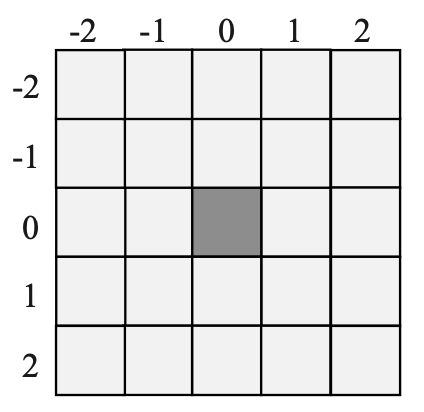
\includegraphics[width=0.60\textwidth]{img/lokaler_operator_maske.jpg}
	\captionof{figure}{Maske eines lokalen Operators nach \citet[S.~52]{handels2000}}
	\label{fig:lokaler_operator_maske}
\end{minipage}

Für die konkrete Betrachtung der Nachbarschaft eines Pixels empfiehlt \citet[S.~52]{handels2000}
eine Maske (Ausschnitt) heranzuziehen, die mit einer Matrix interpretiert werden
kann und die Nachbarschaft eines Pixels abbildet. Abbildung \ref{fig:lokaler_operator_maske}
zeigt eine solche Maske und soll das Verfahren so verdeutlichen. Der grau
hinterlegte Mittelpunkt $P = (0/0)$ ist das aktuell betrachtete Pixel. Die Felder
um die Mitte herum die Nachbarn. Es fällt jedoch auf, dass durch dieses Schema nicht
jede mögliche Ausprägung einer Maske infrage kommt. Um einen Mittelpunkt und
damit ein aktuelles Pixel betrachten zu können, bedarf es eines ungeraden Grades
für $M$. Diese Eingrenzung lässt sich in Gleichung \ref{equ:lokaler_operator}
generisch fassen.

\begin{align}
	\label{equ:lokaler_operator}M_{(2_m+1)x(2_m+1)} & = \begin{bmatrix}k_{11}&k_{12}&k_{13}\\ k_{21}&x&k_{23}\\ k_{31}&k_{32}&k_{33}\\\end{bmatrix} & m \in \mathbb{N}
\end{align}

Die Gleichung \ref{equ:lokaler_operator} beschreibt die mögliche Ausprägung eines
lokalen Operators als Matrix. Dabei sei: $m \in \mathbb{N}\wedge n \in \mathbb{N}$.
Die Variable $x$ beschreibt das aktuell betrachtete Pixel, während $k_{nn}$ die Nachbarn
illustrieren soll. Durch die Gleichung ist auch zu erkennen, dass die Maske des lokalen
Operators beliebig groß werden kann. Eine hohe Ordnung der Operatormatrix ist
jedoch nicht immer von Vorteil, sodass es letzten Endes auf den Anwendungsfall ankommt.

Mit der Technik der lokalen Operatoren können nun unterschiedliche Arten angewendet
werden. \citet[S.~54 - 55]{handels2000} unterscheidet hier in Glättungsfilter,
Mittelwertfilter, Medianfilter, Gaußfilter und Binomialfilter. Alle dieser Filter
bedienen sich einer Operatormaske, um auf Basis der Nachbarelemente einen
statistischen Wert für den Bildpunkt zu erhalten. Um einen genaueren Einblick in
alle Filter zu erlangen, sei an dieser Stelle auf \citet[S.~54 - 55]{handels2000}
verwiesen.

Wie zu Anfang dieses Kapitels beschrieben, ist eine Bildvorverarbeitung (Filterung)
für eine gute Segmentierung des Bildes unerlässlich. So kommt es das auch in der
Visualisierungspipeline nach \citet[S.~50]{handels2000} der zweite Schritt
bereits die Segmentierung einführt. Warum dies so ein wichtiger Bestandteil der Bildanalyse
ist und welche Methoden sich hier bieten, erläutert das folgende Kapitel.
% ---------------------------------------------------------------------------------------

\pagebreak

\subsection{Segmentierung}
\label{subsec:segmentierung} Die Bildsegmentierung oder auch Bildaufteilung genannt,
ist ein wichtiges Teilgebiet der Bildverarbeitung und beschäftigt sich mit der
Bildanalyse. Ihr Ziel ist es, detaillierte beschreibende Bilder aus dem
vorliegenden Originalbild zu berechnen. Dies kann im Falle eines \ac{CT}s der Zahnklinik
an der \ac{LMU} die hervorgehobene Darstellung der Zahnsubstanzen Schmelz und
Dentin sein. \citep[vgl.][S.~359]{lehmann2013bildverarbeitung}. Konkret teilt ein
Segmentierungsverfahren also ein Bild in Teilbereiche auf. Dabei sind die
Teilbereiche in sich bemerkenswert homogen. \citet[S.~1]{ramesh2021} beschreiben,
dass der Prozess der Segmentierung zur Gewinnung wichtiger Informationen dient wie
zum Beispiel die Zahnkaries Ausbreitung. So kommt es, dass \citet[S.~50]{handels2000}
in seiner Visualisierungspipeline die Segmentierung als zweiten Schritt und
damit als zentrales Problem darstellt. \citet[S.~95]{handels2000} und \citet[S.~360]{lehmann2013bildverarbeitung}
beschreiben beide, dass die Bildsegmentierung eines \ac{CT}s für eine gute und
eindeutige ärztliche Diagnose nicht mehr wegzudenken ist. Warum dem so ist,
verdeutlicht die Abbildung \ref{fig:interpretation_einer_ct_aufnahem}.

\begin{figure}[h]
	\centering
	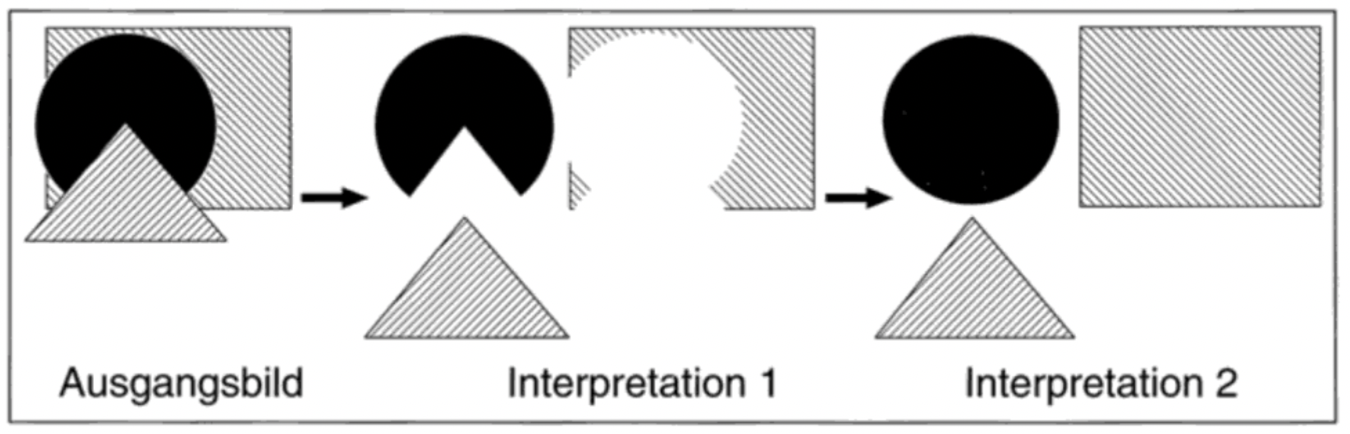
\includegraphics[width=0.8\textwidth]{img/bild_interpretation.jpg}
	\caption{Interpretation einer CT-Aufnahme nach \citet[S.~360]{lehmann2013bildverarbeitung}}
	\label{fig:interpretation_einer_ct_aufnahem}
\end{figure}

Zu erkennen ist das originale Bild (Ausgangslage) und mögliche Interpretationsschritte
(Interpretation 1 und Interpretation 2). \citet[S.~360]{lehmann2013bildverarbeitung}
verdeutlichen mit dieser Abbildung \ref{fig:interpretation_einer_ct_aufnahem},
dass mittels Segmentierung die einzig mögliche Interpretation die Erste ist. Auch
wenn die zweite Interpretation die deutlich logischere ist, kann diese ohne
weitere Forschung nicht bewiesen werden, so \citet[S.~360]{lehmann2013bildverarbeitung}.
Außerdem ist zu erkennen, dass die Abbildung
\ref{fig:interpretation_einer_ct_aufnahem} die Definition einer Segmentierung
belegt. Die Erzeugung inhaltlich zusammengehöriger Regionen werden hier durch die
verschiedenen Formen visualisiert \citep[vgl.][S.~360]{lehmann2013bildverarbeitung}.

Um ein Bild zu segmentieren, gibt es unzählige Möglichkeiten. Für die Auswahl
eines Verfahrens spielt unter anderem der Anwendungsbereich eine wichtige Rolle.
Die Verfahren, die in dieser Arbeit von Wichtigkeit sind, sind die Schwellwertverfahren
\citep[vgl.][S.~361]{lehmann2013bildverarbeitung}.

\pagebreak

\textbf{Schwellwertverfahren} (engl.: thresholding) gehören zu den
Standardwerkzeugen einer Segmentierung, sodass diese die Basis vieler weiterer Verfahren
legen. Bei einer schwellwertbasierten Segmentierung werden die Pixel eines
Bildes anhand von Schwellwerten eingruppiert \citep[vgl.][S.~96]{handels2000}.
Die nachfolgende Gleichung \ref{equ:schwellwertverfahren} soll dies
verdeutlichen.

\begin{align}
	\label{equ:schwellwertverfahren}B(x, y, z) = \begin{cases}1,&\text{falls }t_{\text{unten}}\leq f(x, y, z) \leq t_{\text{oben}}, \\ 0,&\text{sonst}.\end{cases}
\end{align}

$B(x, y, z)$ beschreibt ein Pixel in einem dreidimensionalen Bild, demnach ein
Voxel. Liegen die Werte eines Voxels, also $f(x, y, z)$, innerhalb der beiden Schwellwerte
$t_{oben}$ und $t_{unten}$, dann wird eine 1 zugewiesen. Liegt der aktuell betrachtete
Voxel nicht zwischen den Schwellwerten, so wird eine 0 zugewiesen. Das Ergebnis einer
solchen primitiven Schwellwertsegmentierung ist ein binäres Bild, welches in
Abbildung \ref{fig:binäres_schwellwertverfahren} zu sehen ist.

\begin{figure}[h]
	\centering
	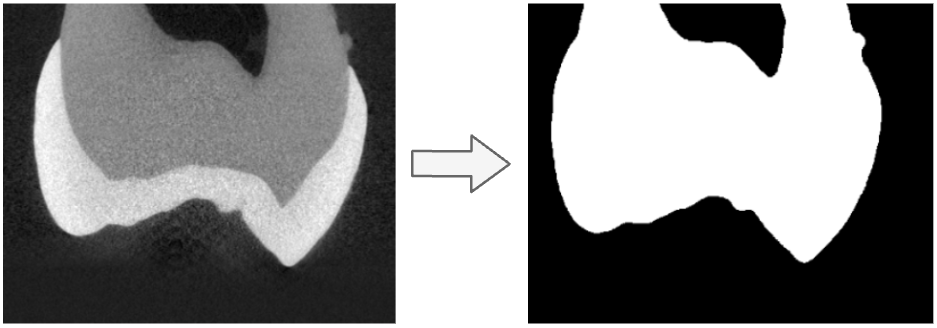
\includegraphics[width=0.8\textwidth]{img/beispiel_schwellwertverfahren.png}
	\caption{Ergebnis eines einfachen Schwellwertverfahrens nach \citet{heck2024} und
	\citet{hoffmann2020}}
	\label{fig:binäres_schwellwertverfahren}
\end{figure}

Zu erkennen ist, dass nach einem einfachen Schwellwertverfahren das Bild nur
noch aus zwei unterschiedlichen Graustufen besteht. Betrachtet man das Ergebnis in
\ref{fig:binäres_schwellwertverfahren} genauer, so ist diese einfache
Segmentierung durchaus erfolgreich verlaufen. Der Grund dafür ist die gute Wahl des
Schwellwerts.

Die interessanteste Frage bei den Schwellwertverfahren ist die Wahl des Schwellwerts
$t$. Dieser entscheidet zwischen einer guten und einer schlechten Segmentierung.
Für die Wahl eines Schwellwerts empfiehlt sich der Blick auf das Bildhistogramm.
Dieses gibt Aufschluss über die Verteilung der Grauwerte in einem Bild \citep[vgl.][S.~361]{lehmann2013bildverarbeitung}.
Verfahren, welche einen guten Schwellwert gewährleistet, ohne dass zu viele
Informationen verloren gehen, sind die Verfahren \textit{Otsu} und \textit{Renyi}.

\pagebreak

\textbf{Das Verfahren nach Otsu} gehört zu den Schwellwertverfahren und bestimmt
den Schwellwert $t$ durch ein statistisches Gütekriterium. Hierzu bedient sich
das Verfahren des Bildhistogramms. Die räumliche Anordnung der Voxel und damit das
tatsächliche Bild, benötigt dieser Algorithmus nicht \citep[vgl.][S.~264]{lehmann2013bildverarbeitung}.

\begin{minipage}{0.40\textwidth}
	Ein solches Histogramm, welches die Grundlage für das Verfahren nach Otsu
	liefert, sei in Abbildung \ref{fig:histogramm} gezeigt. Dies gibt Aufschluss
	über die unterschiedlichen Grauwerte und wie oft sie in einem Bild vorkommen
	\citep[vgl.][S.~264]{lehmann2013bildverarbeitung}. Für eine genauere
	Beschreibung eines Histogramms sei an dieser Stelle auf \citet[S.~42]{burger2009}
	verwiesen.
\end{minipage}
\hfill
\begin{minipage}{0.50\textwidth}
	\centering
	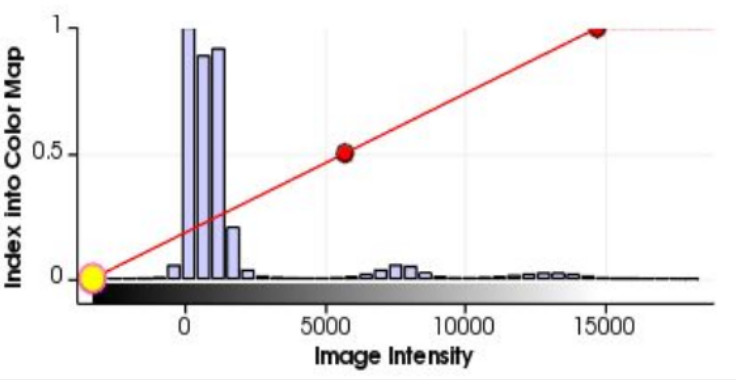
\includegraphics[width=1\textwidth]{img/histogramm.jpg}
	\captionof{figure}{Histogramm einer CT-Aufnahme einer Zahnkrone nach \citet[S.~13]{hoffmann2020}}
	\label{fig:histogramm}
\end{minipage}

Das Otsu-Verfahren teilt die Grauwerte eines Bildes in verschiedenen Klassen ein,
die durch Schwellwerte getrennt werden. Die Klassen können beispielsweise mit
$K_{0}$ bis $K_{n}$ bezeichnet werden, wobei sich dieses konkrete Beispiel auf die
Klassen $K_{0}$ und $K_{1}$ beschränkt. Otsu wählt den Schwellwert $t$, der die Varianz
zwischen den Pixelklassen maximiert und gleichzeitig die Varianz innerhalb jeder
Klasse minimiert \citep[vgl.][S.~264]{lehmann2013bildverarbeitung}. Mathematisch
lässt sich dies wie folgt ausdrücken.
\begin{align}
	t = \text{max }(\sigma_{zw}^{2}/ \sigma_{in}^{2})
\end{align}
$\sigma_{zw}$ bildet die Varianz zwischen den beiden Klassen $K_{0}$ und $K_{1}$
und bildet sich aus den Wahrscheinlichkeiten, mit denen jeder einzelne Grauwert auftritt.
$\sigma_{in}$ hingegen, ist die Varianz innerhalb einer Klasse und entsteht durch
die Addition der Varianzen der einzelnen Klassen. Der Schwellwert $t$ ist nun
der, für den das Verhältnis maximal wird \citep[vgl.][S.~264]{lehmann2013bildverarbeitung}.

Laut \citet[S.~264]{lehmann2013bildverarbeitung} fällt auf, dass dieses
Verfahren vor allem bei bimodalen Bildern zum Einsatz kommt. Ein Bild ist bimodal,
wenn es zwei lokale Maxima aufweist. Vereinfacht gesagt, wenn es zwei lokale
Piecks enthält \citep[vgl.][S.~264]{lehmann2013bildverarbeitung}.

Eine ähnliche Technik für die Bestimmung des Schwellwerts liefert das Verfahren der
Rényi Entropie. Auch hier ist eine Einteilung der Voxel in Klassen vorgesehen.

\pagebreak
% ---------------------------------------------------------------------------------------

\textbf{Das Verfahren nach Rényi} ist ein weiteres Verfahren, das im Laufe dieser
Arbeit noch eine wichtige Rolle spielt. Wie bereits beschrieben gehört es
ebenfalls zu der Gruppe der Schwellwertverfahren und generiert demnach einen
Schwellwert $t$. Wie auch das Verfahren nach Otsu, benötigt Rényi keine
Information über die räumliche Anordnung der Bilder, es genügt das Bildhistogramm.
Dabei ist der optimal Schwellwert $t$ der, der eine maximale Entropie der Bildverteilung
erzeugt. Unter einer Entropie wird ein Konzept verstanden, das eine Unordnung,
Unsicherheit oder den Informationsgehalt innerhalb eines Systems beschreibt, so \citet[S.~102]{bein2006}.
Die Rényi-Entropie ist eine Verallgemeinerung der Shannon-Entropie und hängt von
einem Parameter $q$ ab. Die Entropie misst die Unsicherheit oder den
Informationsgehalt einer Wahrscheinlichkeitsverteilung, welche sich wie folgt ausdrücken
lässt. \citep[vgl.][K.~2]{bromiley2004}.
\begin{align}
	\label{equ:renyi}H_{q}(P) = \frac{1}{1-q}\ln \left( \sum_{i=1}^{N}p_{i}^{q}\right)
\end{align}
Besonderes Augenmerk verdienen hierbei die Parameter $p_{i}$ und $q$, welche die
charakteristischen Eigenschaften der Rényi-Entropie beschreiben. Der Parameter
$p_{i}$ ist die Wahrscheinlichkeit eines jeden Grauwertes im Bild. $i$ symbolisiert
hierbei jeden Grauwert. Wie viele Grauwerte genau betrachten werden sollen
definiert $N$. Die Variable $q$ hingegen beeinflusst die Gewichtung der Wahrscheinlichkeit
$p_{i}$ für jeden Grauwert. Setzt man den Parameter $q$ auf $q = 1$ so lässt
sich mittels Algebra die Shannon-Entropie zeigen \citep[vgl.][K.~2]{bromiley2004}.
Um nun mit der Rényi-Entropie den optimalen Schwellwert für ein Bild zu
berechnen, sieht Rényi ähnlich wie Otsu eine Einteilung in Klassen vor. Die
Einteilung erfolgt mittels des Parameters $N$. So kann nun für jede gebildete Klasse
die Gleichung \ref{equ:renyi} angewendet werden. Die Gesamtentropie des Systems
wird aus den beiden Teilentropien der jeweiligen Klassen bestimmt\citep[vgl.][K.~2]{bromiley2004}.
\begin{align}
	H_{q}(T) = H_{q}(P)^{(1)}+ H_{q}(P)^{(2)}
\end{align}
Um nun den optimalen Schwellwert $t$ bestimmen zu können muss der Wert genommen werden,
bei dem die Gesamtentropie des Systems maximal ist. Dieser Sachverhalt lässt sich
wie folgt ausdrücken \citep[vgl.][K.~2]{bromiley2004}.
\begin{align}
	t = max(H_{q}(T))
\end{align}
Gegen Ende des Kapitels konnte ein grundlegendes Verständnis über die anatomische
Segmentierung einer Zahn-\ac{CT}-Aufnahme gewonnen werden. Um dieses Verfahren,
wie von der Fragestellung gefordert, für den klinischen Alltag zugänglich zu machen,
ist eine benutzerfreundliche Lösung erforderlich. Im folgenden Kapitel wird daher
die automatische Segmentierung mit 3D Slicer behandelt, einer etablierten
Plattform, die eine effiziente Integration und Nutzung des Verfahrens ermöglicht.
% ---------------------------------------------------------------------------------------
	\chapter{Automatische Segmentierung mittels 3D Slicer}
\label{sec:3d_slicer} 3D Slicer ist eine Open-Source-Plattform, die speziell für
die Verarbeitung von Bilddaten im medizinischen Kontext eingesetzt wird. Dabei wird
sie von einer aktiven Community regelmäßig gewartet und weiterentwickelt \citep[vgl.][]{slicer2024},
\citep[vgl.][S.~1325]{fedorov2012slicer}. Für Slicer gibt es offiziell keine Nutzungsbeschränkung.
Jedoch sei auch gesagt, dass 3D Slicer nicht für die klinische Nutzung zugelassen
ist. \citet[S.~1331]{fedorov2012slicer} machen deutlich, dass 3D Slicer
ausschließlich für die Forschung gedacht ist. Um einen ersten Überblick über die
Komponenten von Slicer zu erlangen, soll die Abbildung
\ref{fig:3d_slicer_oekosystem} betrachtet werden.

\begin{figure}[h]
	\centering
	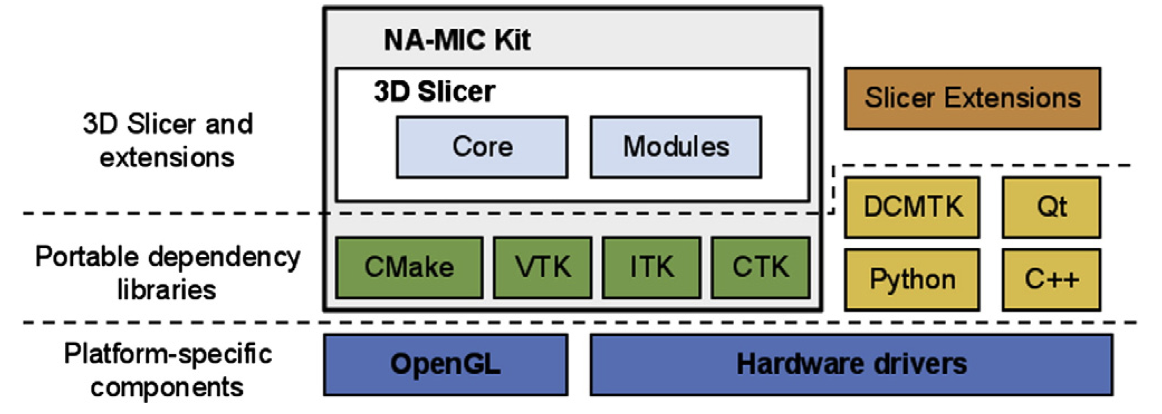
\includegraphics[width=1\textwidth]{img/3d_slicer_overview.jpg}
	\caption{3D Slicer Ökosystem nach \citet[S.~1326]{fedorov2012slicer}}
	\label{fig:3d_slicer_oekosystem}
\end{figure}

\citet[S.~1326]{fedorov2012slicer} teilt mit der Abbildung
\ref{fig:3d_slicer_oekosystem} die Plattform in drei Schichten auf. Auf der Obersten
wird klar, dass 3D Slicer aus der Kernanwendung und den installierbaren Modulen
besteht. Neben den bereits vorhandenen Modulen können, von externen Entwicklern
Module über die Slicer Erweiterung entwickelt und bereitgestellt werden. Um eine
Weiterentwicklung möglich zu machen hat Slicer eine Reihe von Abhängigkeiten,
die jedoch portabel gehalten werden. Auf der untersten Schicht sind die Plattformspezifischen
Anforderungen zu sehen, die Slicer erfüllen soll. So kommt es, dass das 3D
Slicer Ökosystem sich durch einige Kriterien auszeichnet, die es besonders attraktiv
für die Bearbeitung von medizinischen Bilddaten machen. Zu den wichtigsten
Vorteilen gehört die Tatsache, dass die Software kostenfrei verfügbar ist.
Darüber hinaus bietet sie eine umfassende Plug-in-Infrastruktur, die über den sogenannten
\textit{Extension-Manager} zugänglich ist. Dies ermöglicht eine einfache Erweiterung
der Funktionalitäten nach Bedarf. Ein weiteres herausragendes Merkmal ist die
Möglichkeit, Skripte direkt in der integrierten Python-Konsole auszuführen, was
eine flexible und effiziente Automatisierung von Prozessen ermöglicht. Schließlich
ist 3D Slicer besonders für seine Vielseitigkeit bekannt, da es medizinische
Bilddaten aus sämtlichen Bereichen der Medizin verarbeiten kann.

3D Slicer hat für alle diese Punkte jeweils eine Lösung entwickelt, wobei der erste
Punkt durch die Open-Source-Philosophie schon gegeben ist. Die folgenden
Abschnitte decken diese Lösungen ab und bilden so eine erste Grundlage für die
Entwicklung mit 3D Slicer.
% ---------------------------------------------------------------------------------------

\section{Plug-in-Infrastruktur}
Der wohl bedeutendste Punkt ist die Plug-in-Infrastruktur, welche Slicer von sich
aus mitbringt. Um dieses Konzept genauer zu beleuchten, teilt man die Plattform am
besten in zwei Teile auf, die Kernanwendung und die Module, welcher jeder Anwender
personalisiert installieren oder deinstallieren kann. Diese Module werden als
\textit{Slicer lodabel module} bezeichnet \citep[vgl.][S.~1332]{fedorov2012slicer}.
Slicer realisiert die Struktur durch den \textit{Extension Manager}, welcher durchaus
vergleichbar ist mit einer Art App-Store. Über diesen können bequem und mit
wenig Klicks die gewünschten Erweiterungen in das Kernsystem installiert werden.
Neben der Möglichkeit Module zu installieren bietet Slicer noch die Möglichkeit eigenen
Module zu bauen und Sie im \textit{Extension Manager} zu veröffentlichen. Diese werden
als \ac{SEM} bezeichnet. Abbildung \ref{fig:3d_slicer_extension_index} soll diesen
Vorgang verdeutlichen \citep[vgl.][]{slicer2024}.

\begin{figure}[h]
	\centering
	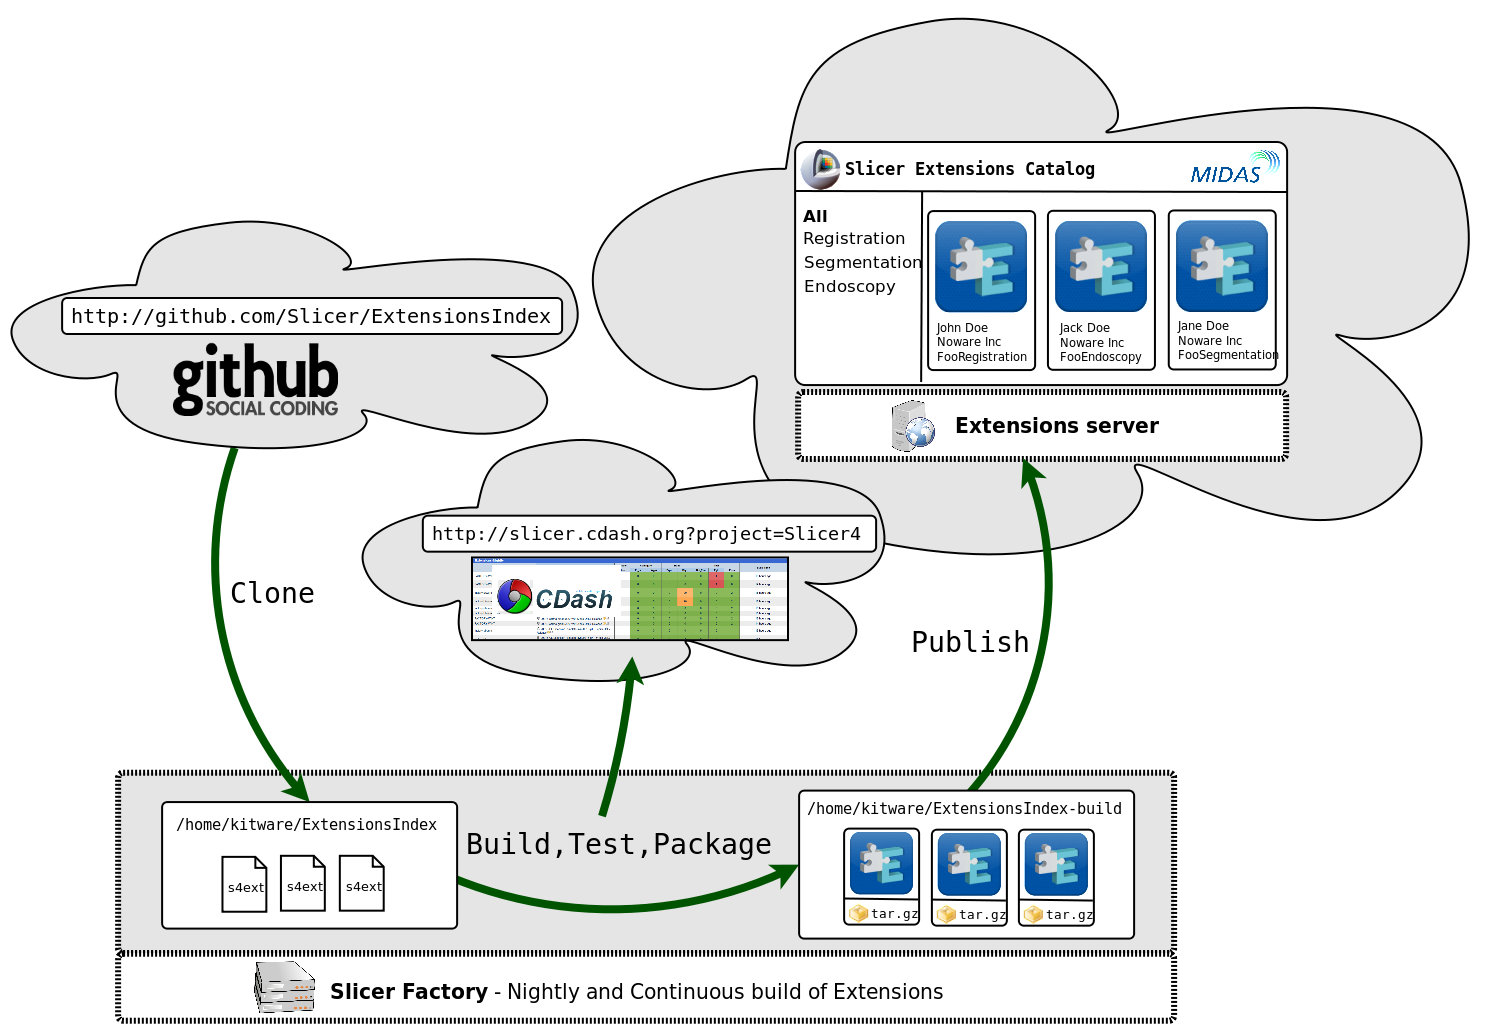
\includegraphics[width=0.7 \textwidth]{img/slicer_extention_index.png}
	\caption{Funktionsweise der Plug-in-Infrastruktur von 3D Slicer nach \citet{extensionsIndex2024}}
	\label{fig:3d_slicer_extension_index}
\end{figure}

Slicer realisiert dies, indem die Plattform über ein zusätzliches Repository
verfügt, dass sich \href{https://github.com/Slicer/ExtensionsIndex?tab=readme-ov-file}{\textit{ExtensionIndex}}
nennt. Dieses öffentliche Repository ist eine Auflistung aller \ac{SEM}. Die
Auflistung erfolgt durch eine Reihe an \ac{JSON} Dateien, die auf die
Repositorien der einzelnen Entwickler verweisen. Dieser \href{https://github.com/Slicer/ExtensionsIndex?tab=readme-ov-file}{\textit{ExtensionIndex}}
ist über die Slicer Factory an den Extention Server und damit auch an den Extention
Manager angebunden. Die Slicer Factory ist ein System, das aus einem Slicer Extention
Repository ein lauffähiges Build erstellt, welches in den Extention Katalog
eingebunden werden kann. Ist eine Erweiterung in dem Erweiterungskatalog gelistet,
so sorgt der \textit{Extension Manager} dafür, dass die von der Slicer Factory
erstellt Build-Datei installiert werden kann.

Während die Module von Slicer gebaut werden, werden parallel auch immer die Tests
für die Kernanwendung ausgeführt. Diese sind über ein Dashboard einsehbar. So wird
sichergestellt, dass keines der Module einen Fehler im Kernsystem verursacht. Außerdem
ist so für alle Benutzer von Slicer transparent einsehbar, in welchem Zustand
sich die Software gerade befindet. Die Kernanwendung von 3D Slicer folgt einem Entwurfsmuster,
dass sich \ac{MVC} nennt. Bei der Erstellung einer \ac{SEM} soll dieser Ansatz ebenfalls
gepflegt werden. Eine High Level Betrachtung der Softwarearchitektur von 3D
Slicer bietet \cite[S.~1332]{fedorov2012slicer} mit der Abbildung
\ref{fig:3d_slicer_architektur}.

\begin{figure}[h]
	\centering
	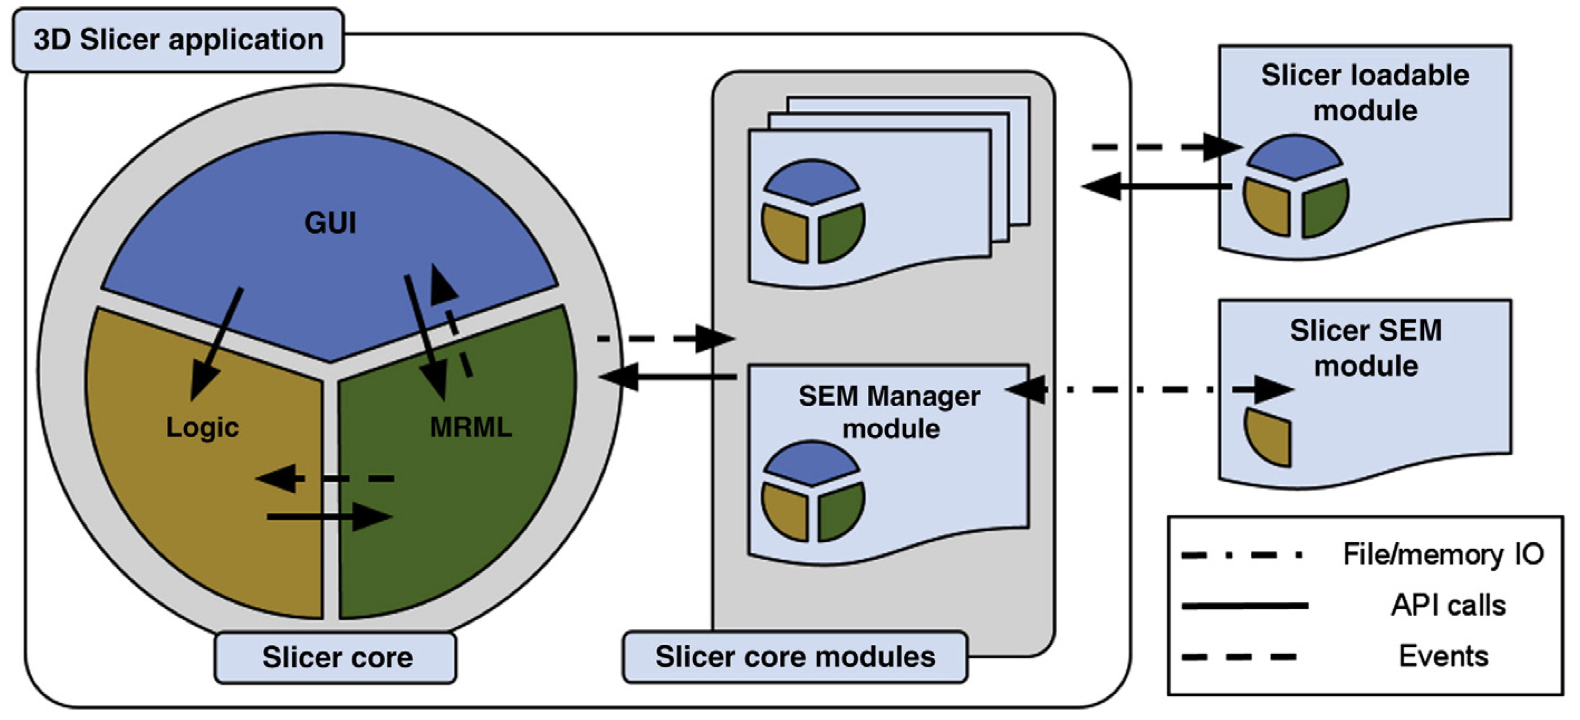
\includegraphics[width=0.7\textwidth]{img/3d_slicer_architektur.jpg}
	\caption{3D Slicer High Level Architektur nach \citet[S.~1332]{fedorov2012slicer}}
	\label{fig:3d_slicer_architektur}
\end{figure}

Das Zusammenspiel zwischen \ac{MRML}, \ac{GUI} und der Logik bilden das MVC-Pattern
in der Kernanwendung. Das identische Pattern spiegelt sich auch in den einzelnen
Modulen von Slicer wieder. So wird sichergestellt, dass ein Softwareentwicklungsparadigma
eingehalten wird, was sich \textit{separation of concerns} nennt. Die Kapselung
von zusammengehöriger Logik. Bei der Erstellung einer eigenen Erweiterung ist die
Idee, dass nur die Logik implementiert werden muss und die komplexe Architektur
von Slicer erstmal nicht relevant ist.

Jedoch bietet sich in Slicer nicht nur die Möglichkeit eigene Erweiterungen zu
erstellen, es lässt sich hierfür auch die integrierte Python-Konsole nutzen.
% ---------------------------------------------------------------------------------------

\section{Python-Umgebung}
\label{subsec:pythob_umgebung} 3D Slicer bringt eine integrierte Python-Konsole mit,
über die mit der Datenstruktur interagiert werden kann. So ist es möglich,
Python-Skripte direkt in der Konsole auszuführen. Um dies zu realisieren, bringt
Slicer mit der Installation im jeweiligen Betriebssystem eine eigene Python-Umgebung
mit. Dieses sieht wie folgt aus.

\begin{center}
	\texttt{./Slicer/bin/PythonSlicer}
\end{center}

Diese Python-Umgebung verfügt über alle notwendigen Abhängigkeiten und Pakete. Bei
der Entwicklung eines \ac{SEM} kann dann auf das \ac{PyPi} in der integrierten Python-Umgebung
zurückgegriffen werden. So kommt es, dass für eine Entwicklung mit Slicer keine eigene
Python-Umgebung auf der lokalen Maschine installiert sein muss. Slicer bringt
hier alles mit. Für die Anwender, die eine terminal basierte Bearbeitung
vorziehen, besteht diese Möglichkeit nach wie vor.

Für den letzten charakteristischen Punkt von Slicer aus Kapitel \ref{sec:3d_slicer}
führt der nächste Abschnitt in die durchaus komplexe Datenstruktur \ac{MRML} ein,
die bei einer Entwicklung mit Slicer unausweichlich zu berücksichtigen ist.
% ---------------------------------------------------------------------------------------

\section{MRML-Datenstruktur}
\label{subsec:mrml_datenstruktur} Die \ac{MRML}, gesprochen \textit{"Murlm"} ist
ein Datenmodell, das dafür entwickelt wurde, alle möglichen Bilddaten zu
visualisieren und zu speichern, die für einen klinischen Zweck Einsatz finden \citep[vgl.][]{slicer2024}.
Laut \citet{slicer2024} wurde die \ac{MRML}-Datenstruktur völlig unabhängig von der
Slicer Kernanwendung entwickelt. Dies ermöglicht ein Portieren der Datenstruktur
auf andere Softwareapplikationen. Da Slicer die einzig große Plattform ist, die
diese Datenstruktur nutzt, wird der Quellcode für \ac{MRML} im Repository von 3D
Slicer gewartet und weiterentwickelt, so \citet{slicer2024}. Durch den Artikel von
\citet[S.~1331]{fedorov2012slicer} wird klar, dass \ac{MRML} mehr ist also nur
eine Datenstruktur. Sie beschreiben \ac{MRML} als Szenenorganisator von Bilder, Annotationen,
Layouts und Anwendungsdaten. \citet[S.~1327]{fedorov2012slicer} beschreiben die
\ac{MRML}-Datenstruktur als Schlüsselkomponenten innerhalb von 3D Slicer. Dies
ist auf die Softwarearchitektur von Slicer zurückzuführen, die in Abbildung \ref{fig:3d_slicer_architektur}
beschrieben wurde. Die Kernanwendung von Slicer arbeitet wie bereits beschrieben
nach dem \ac{MVC}-Pattern. \ac{MRML} übernimmt hier den Teil des \textit{Models
(M)} und bildet damit den Grundstein der Anwendung \citep[vgl.][S.~1332]{fedorov2012slicer}.
\citet{slicer2024} und der Artikel von \citet[S.~1327]{fedorov2012slicer}
beschreibt \ac{MRML} als \ac{XML}-Format. Wird also eine \ac{MRML}-Szene
gespeichert, so folgt eine Speicherung als \ac{MRML}-Datei und damit unter der
Haube als \ac{XML}-Datei. Dabei wird laut \citet{slicer2024} nur eine Referenz auf
das Bild gespeichert. Die zu bearbeitende Aufnahme selbst wird nicht innerhalb
einer \ac{MRML}-Datei abgespeichert. \ac{MRML} zeichnet sich vor allem dadurch aus,
dass es eine Vielzahl an Dateiformaten akzeptiert. Alle Formate, die für einen
klinischen Zweck verarbeitet werden, können durch \ac{MRML} unterstützt werden. Um
dies zu gewährleisten, ist die \ac{MRML}-Szene in sogenannte Knoten (engl.:
nodes) aufgeteilt. Die Basistypen für einen Knoten folgen der \citet{slicer2024}
und sind in der folgenden Aufzählung zu sehen.

\begin{minipage}{0.45\textwidth}
	\begin{itemize}
		\item Data node

		\item Display node

		\item Storage node

		\item View node
	\end{itemize}
\end{minipage}
\hfill
\begin{minipage}{0.45\textwidth}
	\begin{itemize}
		\item Plot node

		\item Subject hierarchy node

		\item Sequence node

		\item Parameter node
	\end{itemize}
\end{minipage}

Wird also ein Bild in eine \ac{MRML}-Szene geladen, so speichert Slicer die
unterschiedlichen Eigenschaften eines Bildes in unterschiedlichen Knoten. So werden
Beispielsweise Basiseigenschaften einer Probe im \textit{Data node} gespeichert,
wo hingegen ein \textit{Storage node} beschreibt wie ein Bild auf der Festplatte
gespeichert wird. In \textit{Display node} werden die Eigenschaften zur
Darstellung eines Bildes hinterlegt. Der Hintergrund für die Speicherung von Probendaten
in unterschiedlichen Knoten ist, dass beispielsweise dasselbe Bild in
unterschiedlichen Formaten vorliegt oder ein und dasselbe Bild auf zwei
unterschiedliche Arten visualisiert werden soll. So kann sich beispielsweise eine
Struktur wie in Abbildung \ref{fig:3d_slicer_class} ergeben.

\begin{figure}[h]
	\centering
	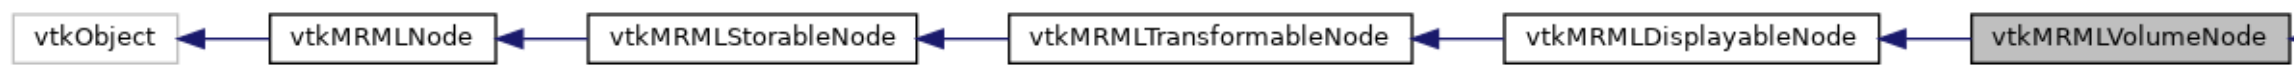
\includegraphics[width=1\textwidth]{img/slicer_class_index.jpg}
	\caption{Verkettung der einzelnen Knoten in der MRML-Datenstruktur nach
	\cite{slicer2024}}
	\label{fig:3d_slicer_class}
\end{figure}

Die Informationen in einem Bild werden also über diese Typen aufgeteilt und je
nach Sinn abgespeichert. Möchte man demnach auf die bestimmte Informationen in einer
Probe zugreifen. So kann diese Information über den Aufruf bestimmter Methoden
erfolgen

\begin{lstlisting}[
	language={python},
	caption={Auslesen der Informationen aus den verschiedenen Knoten},
	label={lst:_auslehsen_nodes}]
# data node - vtkMRMLVolumeNode
currentVolume.GetImageData()
# storage node - vtkMRMLStorableNode
currentVolume.GetStorageNode()
# display node - vtkMRMLDisplayableNode
currentVolume.GetDisplayNode()
\end{lstlisting}

Wie die Kommentare in Listing \ref{lst:_auslehsen_nodes} bereits zeigen, gibt es
noch eine Besonderheit von \ac{MRML}. Damit eine Verwaltung aller Dateiformate möglich
ist, bedient sich \ac{MRML} einiger Tools, die sich bereits etabliert haben. Die
Wichtigsten sind hierbei \ac{VTK} und \ac{ITK} \citep[vgl.][K.~1.1]{vtk2006}, \citep[vgl.][K.~1.1]{itkguide2015}.
Die beiden Tools sind echte Riesen in ihrer Branche. \ac{MRML} nutzt diese, um
einige Dateiformate zu lesen und zu schreiben. Durch das Betrachten der \ac{MRML}-Szene
wird klar, dass Slicer hierdurch viele Möglichkeiten bietet. Speziell für die
effiziente Speicherung der Proben in einer Szene durch die unterschiedlichen
Knotentypen. Ein besonderer Knoten, der gleichzeitig auch die Brücke zu der
interaktiven Benutzerschnittstelle von Slicer baut, ist der \textit{Parameter
node}.

Mit dem Ende dieses Kapitels wurden alle wichtigen theoretischen Grundlage
besprochen, die notwendig sind um die anatomische Segmentierung über ein 3D Slicer
Modul bereitzustellen. Bevor die konkrete Methodik thematisiert wird, die für die
Entwicklung des Moduls angewendet wird, sollen im nächsten Kapitel kurz die
Rahmenbedingungen gesetzt werden, innerhalb deren entwickelt werden soll.
% ---------------------------------------------------------------------------------------
	\chapter{Entwicklungsumgebung}
\label{chap:entwicklungsumgebung} Da bereits ein Framework feststeht, mit dem
gearbeitet werden soll, ist keine weitere Forschung nötig, um die richtige
Programmiersprache auszuwählen. Jedoch gibt es eine kleine Auswahl zu treffen.
3D Slicer unterscheidet zwischen zwei Arten von Modulen, die \ac{CLI}-Module, welche
in der Sprache C++ geschrieben werden und die \textit{Scripted Moduls}, die eine
Python Implementierung verlangen. Da die anatomische Segmentierung ohnehin in
einem IPython-Notebook bereitliegt, fiel die Wahl hier auf die Scripted Moduls.
So kann auch die breite Palette der Python-Pakete genutzte werden. Für eine detaillierte
Beschreibung des Frameworks selber sei an dieser Stelle auf das Kapitel \ref{sec:bildbearbeitung}f
verwiesen, indem das Framework und alle zugehörigen Eigenheiten noch genauer beschrieben
wurden. Um den Entwicklungsprozess etwas zu vereinfachen, wurde während der Entwicklung
auf ein Modul von Slicer zurückgegriffen, das speziell für Entwickler entworfen
wurde. Die Abbildung \ref{fig:entwicklungsumgebung} verdeutlicht dieses Tool.

\begin{figure}[h]
	\centering
	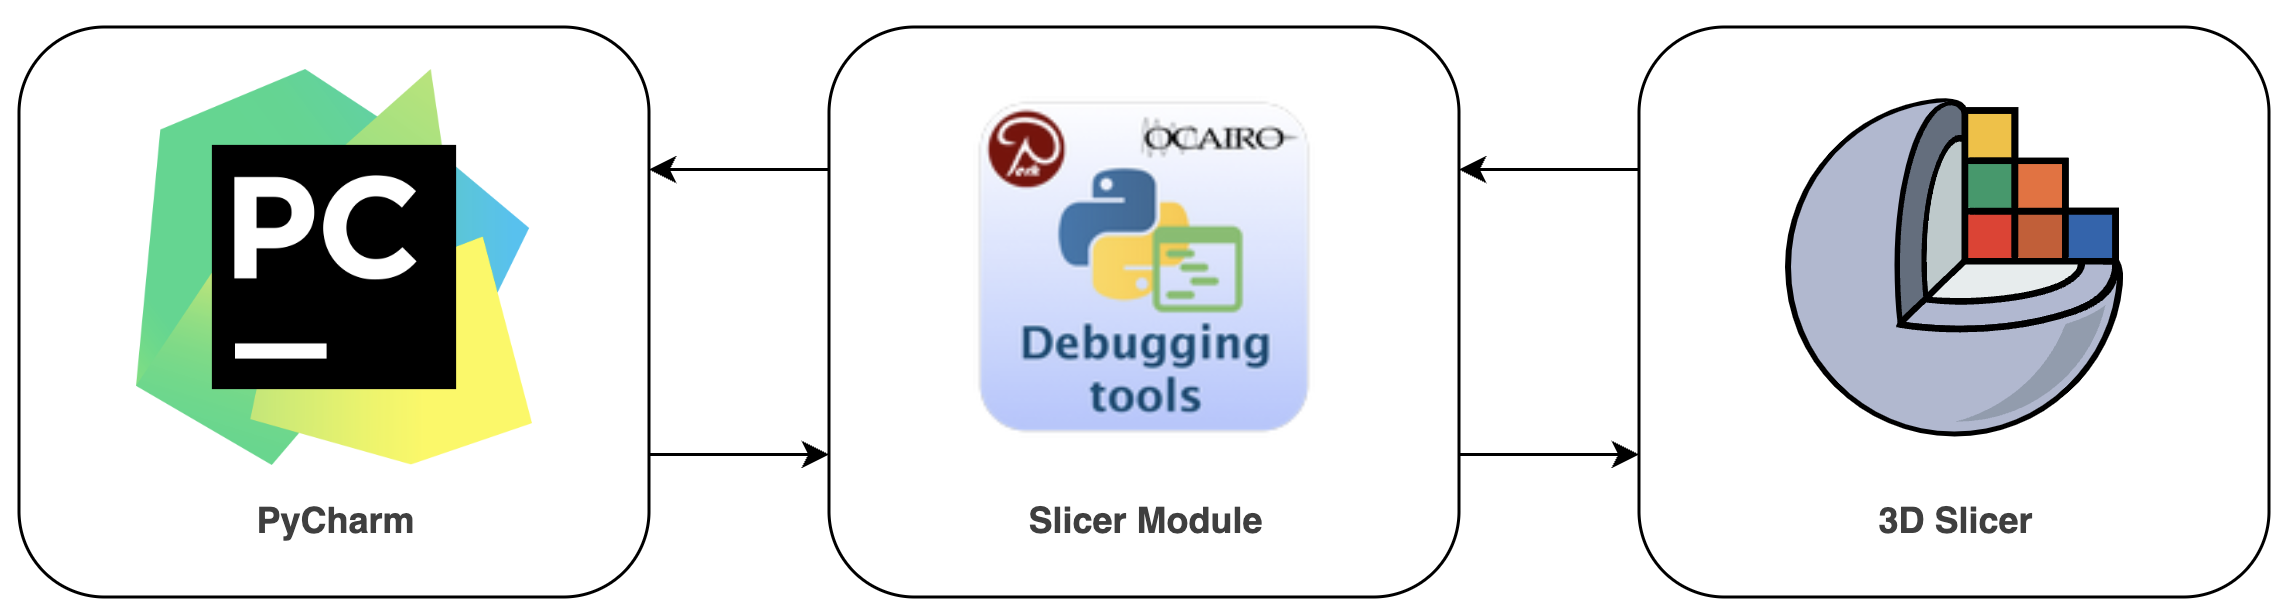
\includegraphics[width=0.6\textwidth]{img/Entwicklungsumgebung.png}
	\caption{Umgebung während der Entwicklung mit 3D Slicer und PyCharm}
	\label{fig:entwicklungsumgebung}
\end{figure}

Mit dem Debugging Tool lässt sich eine gewohnte Umgebung reproduzieren, in der der
Quellcode Schritt für Schritt analysiert werden kann \citep[vgl.][]{slicerdebuggingtools}.
Speziell bei der Fehlersuche ist dieses Tool eine sehr gute Unterstützung. Die
Abbildung beschreibt weiter, das als Umgebung für das Erstellen des Programmcodes
die Software Pycharm verwendet wird. Pycharm ist eine Lösung der Firma Jetbrains,
für das Erstellen von Python-Quellcode. Dieses Tool bietet eine breite Palette
an Funktionalitäten, die das Erstellen von Software vereinfachen und als \textit{State
of the Art} bezeichnet werden kann \citep[vgl.][]{jetbrains2024}.

Für die Interaktion mit der Slicer Kernanwendung stellt der Python-Interpreter das
Paket \texttt{slicer} zur Verfügung. Hierdurch lassen sich diverse Mechanismen steuern.
Wichtig ist hierbei, dass das Paket \texttt{slicer} nicht auf \ac{PyPi} zu finden
ist. Es ist nur in der Python-Umgebung vorhanden, die mit der Slicer Installation
einhergeht. Neben dem Paket \texttt{slicer} sind noch viele weitere Pakete verfügbar,
die sich in der medizinischen Bildbearbeitung durchgesetzt haben. Für eine komplette
Auflistung aller Python-Pakete sei an dieser Stelle auf die Dokumentation von Slicer
verwiesen \citep[vgl.][]{slicer2024}.

Auch die Versionierung des Quellcodes wurde von Anfang an in den
Entwicklungsprozess integriert. Da die Software ohnehin über ein öffentliches GitHub-Repository
in Slicer eingebunden wird, diente dieses zugleich als zentrales Werkzeug zur
Versionskontrolle. Im Hintergrund kommt dabei selbstverständlich Git zum Einsatz.
Den Link zum öffentlichen Repository kann dem Anhang entnommen werden.

Damit während der Entwicklung auch Teilbereiche der Software bereits getestet
werden können, werden Testdaten benötigt. Bei diesen Testdaten handelt es sich
um originale Mikro-\ac{CT}-Aufnahmen als \ac{ISQ}. Diese wurden auf einem Server
an der \ac{LMU} in München bereitgestellt. Der Zugriff auf den Server erfolgt über
den \textit{x2goclient}. Heruntergeladen wurden die Daten über eine \ac{SSH}
Verbindung heruntergeladen werden. Bei den Mikro-\ac{CT}-Bildern handelt es sich ausschließlich
um Aufnahmen der Zahnkrone. Mit dem Zugriff auf den Server an der \ac{LMU} konnten
auch diverse Pythonumgebungen zum Verarbeiten von Daten genutzt werden. Dies war
in erster Linie für ein Nachvollziehen und Verstehen der anatomischen
Segmentierung hilfreich.

Neben der eigentlichen Umgebung von Slicer und den Entwicklerwerkzeugen steht
zur Entwicklung auch ein Python Paket zur Verfügung, das von Herrn Prof. Rösch
speziell für die Klinik an der \ac{LMU} erstellt wurde. Dieses Tool beinhaltet
diverse Funktionalität für das Verarbeiten von medizinischen Bilddaten. Speziell
für die Mikro-\ac{CT}-Aufnahmen der Klinik.

Nachdem die Entwicklungsumgebung definiert und eingerichtet wurde, kann nun auf die
konkrete Methodik eingegangen werden, die zur Umsetzung dieser Schnittstelle
verwendet wird. Dabei werden sowohl die Anforderungen an die Erweiterung beschrieben,
also auch die konzeptionellen Überlegungen detailliert beschrieben.

% ---------------------------------------------------------------------------------------
	\chapter{Methodik}
\label{chap:methodik} test
	\chapter{Ergebnisse}
\label{chap:ergebnisse}

\section{Metainormationen}
Hier steht eine allgemine Beschreibung der Extension Name, ersteller, ....

\section{Konzeptionen}
Diagramme

\section{Implementierungen}
Wichtige Codeausschnitte

\section{Recherche zum Stand der Kunst}
\label{sec:recherche} Für die Recherche zu den verschiedenen Teilaufgaben ist
die Dokumentation der Open Source Plattform 3D Slicer eine wichtige Ressource
\cite[vgl.]{[}]{slicer2024}. Diese zeigt bereits etablierte Verfahren und einen \textit{Best
Practise} Ansatz. Auch das \citet{extensionsIndex2024} Repository ist eine
wichtige Quelle, da so ein Einblick in andere Lösungen möglich ist. So kommt es,
das nach ausführlicher Recherche zu den Teilaufgaben UI-Design, Pseudo-Extension,
Kapselung Hoffmann, Speicherung Parameter, Dokumentation und Test bereits Lösungen
existieren. Bei diesen Lösungen handelt es sich jedoch nicht um konkrete
Ergebnisse, sondern vielmehr um einen Leitfaden zur Lösung der Teilaufgabe. Die
Recherche hat demnach ergeben, dass diese Teilprobleme im Kontext der 3D Slicer Umgebung,
nicht das erste Mal zutage treten und Lösungswege existieren.

\begin{minipage}{0.40\textwidth}
	Für ein \textbf{UI Design} wird sehr empfohlen, bereits etablierte 3D Slicer Extensions
	als Orientierung zu nutzen. Eine sehr gute Orientierung bietet das Modul
	\textit{Transforms}, das in Abbildung \ref{fig:module_example} zu sehen ist. Zu
	Erkennen ist, dass die UI mittels Collapsible Buttons in verschiedenen Gruppen
	unterteilt wird. Ohne in die verschiedenen Gruppen hineinzublicken, lässt sich
	gut abschätzen, welche Parameter wo zu erwarten sind. Dies ermöglicht dem
	Benutzer ein isoliertes Betrachten der unterschiedlichen Funktionen in diesem
	Modul und so eine gute Benutzerfreundlichkeit.
\end{minipage}
\hfill
\begin{minipage}{0.50\textwidth}
	\centering
	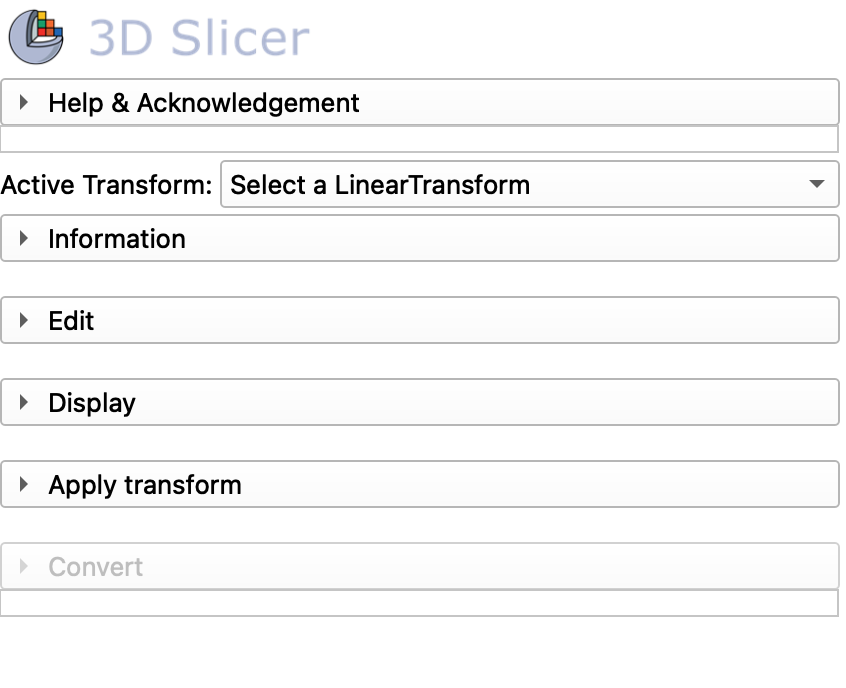
\includegraphics[scale=0.50]{img/modul_example.jpg}
	\captionof{figure}{Das Modul Transforms als Beispiel einer etablierten UI für eine Slicer Extension | Screenshot aus 3D Slicer}
	\label{fig:module_example}
\end{minipage}

Für die Extension, welche in der vorliegenden Arbeit erstellt werden soll, wird genau
dieser Ansatz gepflegt und somit eine gute Benutzbarkeit des Moduls gewährleistet.
Die speziellen wünsche der konkreten Benutzergruppe sollen jedoch nicht zu kurz
kommen.

Für das Erstellen einer \textbf{ersten funktionierenden Extension} bietet Slicer
eine sehr gute Hilfe. 3D Slicer hat hierfür ein eigenes Modul entwickelt, das sich
\textit{Extention Wizard} nennt. Dieses Modul gibt eine gute Einführung in die Entwicklung
mit Slicer. Hiermit lässt sich mittels Leitfaden eine erste Demo Extension
erstellen, die sich bereits gut in 3D Slicer einfügt. Diese Lösung könnte als
Abstraktionsschicht betrachtet werden, da durch dieses Modul im ersten Schritt nahe
zu keine Kenntnisse über die Kernanwendung von Slicer nötig sind. Der
Extentionwizard ist wie folgt zu finden:

\texttt{Modules -> Developer Tools -> Extension Wizard}

Für \textbf{die Kapselung} einer bestimmten Einheit von Code, sieht Slicer eine
Bibliothek innerhalb der Extention vor, so beschreibt es die \citet{slicer2024}.
Das Listing \ref{lst:3d_slicer_projektverzeichnis} zeigt, wo eine Bibliothek
innerhalb einer Extention einzuordnen ist, hier als \texttt{MyLib} zu sehen. Innerhalb
dieses Ordners können sich weitere Module befinden, die als einfache Python-Files
abgelegt werden. Zu beachten ist, dass in jeder Bibliothek eine \texttt{\_\_init\_\_.py}
hinzugefügt wird, sodass dieser Ordner auch entsprechend verwendet werden kann.

\begin{lstlisting}[
    language={python},
    caption={Prinzipeller Aufbau eines Projektes für eine Slicer Extension nach Slicer (2024)},
    label={lst:3d_slicer_projektverzeichnis}]
|-- CMakeLists.txt
|-- MyLib
|   |-- __init__.py
|   |-- cool_maths.py
|   |-- utils.py
|-- MyExtension.py
\end{lstlisting}

Für die Teilaufgabe zur \textbf{Speicherung der Parameter} nutzt Slicer eine
Technik, das durchaus als eines der Kernfunktionen beschrieben werden kann. Die
Rede ist hier von der Klasse \texttt{ParameterNodeWrapper}. Dieser wurde bereits
zu einem früheren Zeitpunkt in dieser Arbeit beschrieben. Für die Funktion dieser
Lösung sei auf den Abschnitt \ref{subsec:benutzerschnitstelle} Benutzerschnittstelle
verwiesen.

Sowohl das \textbf{Benutzerhandbuch}, also auch die technische Dokumentation einer
Slicer Extension wird immer in der \texttt{README.md} des jeweiligen Repository
hinterlegt. In der Extension selber sieht Slicer keine umfangreiche Dokumentation
vor. Es wird lediglich via Link auf die Dokumentation im Repository verwiesen
und eine kurze Einführung gegeben. Auch hier gibt es wieder etablierte Designs,
die als Vorlage verwenden werden können. Die \citet{slicer2024} erwähnt hier
unter anderem das Module
\href{https://github.com/lassoan/SlicerSegmentMesher}{SegmentMesher} als gutes
Beispiel.

Für die Letzte Teilaufgabe, das \textbf{Testen}, gibt die Dokumentation von 3D Slicer
ebenfalls eine konkrete Struktur vor. Ist ist also nicht nötig eigenen Verfahren
zu entwickeln. Für die Softwaretests stell Slicer eine eigene Klasse innerhalb der
Slicer Bibliothek bereit, die alle wichtigen Funktionen enthält, um konkrete Testfälle
zu schreiben. Die Klasse Trägt den Namen \textsl{ScriptedLoadableModuleTest} und
kann als Elternklasse für einen Testfall verwendet werden.

\begin{lstlisting}[
    language={python},
    caption={Aufbau einer Testklasse zum ausführen von Unittest nach \citet{slicer2024}},
    label={lst:3d_slicer_test_class}]
class MyExtensionTest(ScriptedLoadableModuleTest)
    def setUp(self):
      # do something befor a test
    def runTest(self):
      # execute your test case here
    def testMyExtension1(self):
      # write your test case here
\end{lstlisting}

Im Listing \ref{lst:3d_slicer_test_class} ist zu sehen, dass sich die Klasse in drei
Teil aufteilt, die Methode \texttt{setUp()}, die als Vorbedingung dient, die Methode
\texttt{runTest()}, die über die UI getriggert werden kann um die Test zu starten
und die konkreten Textfälle, die in selbst definierten Methoden geschrieben
weden können. Als Beispiel sie hier die Methode \texttt{testMyExtension1()}
gezeigt.

Im Laufe dieses Kapitels wurde klar, dass es für einige der Teilaufgaben bereits
Lösungen oder Lösungsansätze gibt, die zu etwas weniger Entwicklungsarbeit
führen. Jeodch trifft dies nicht auf alle Punkte zu, sodass sich der nächste
Abschnitt mit der Erarbeitung von konkreten Lösungsansäätzen für die noch nicht
behandelten Teilaufgaben beschäftigt.
% ---------------------------------------------------------------------------------------

\section{Erarbeiten von Lösungsansätzen}
\label{sec:lösungsansätze} hier geht es um Brainstorming

\textbf{Architekturdesign}

\textbf{Single Prozess}

\textbf{Batch Prozess}

% ---------------------------------------------------------------------------------------

\section{Auswahl von Lösungsansätzen}
	\chapter{Evaluierung}
\label{subsec:evaluierung} Neben der Implementierung der Features wurden auch diverse
Tests durchgeführt, die eine Bewertung der Ergebnisse möglich machen. Hierzu wurden
Softwaretests, Benutzertests und Messungen durchgeführt. Dieses Kapitel beschäftigt
sich mit den verschiedenen Tests und deren Auswertung. Begonnen wird mit einer
Analyse der Softwaretests, gefolgt von Laufzeitmessungen. Abschließend werden
die Anwendungsfälle des Tooth Analyser näher beleuchtet und auf die
Limitierungen der Anwendung eingegangen.

\section{Softwaretests}
\label{subsec:softwaretests} Betrachtet man die Dokumentation von Slicer genauer,
so fällt auf, dass dies eine recht starre Struktur für die Implementierung von
Tests vorgibt. Dabei ist jedoch nicht festgelegt, welche Art von Tests verwendet
werden soll. Im Rahmen des Tooth Analyser wurden hier ausschließlich Unittest implementiert,
welche die einzelnen Einheiten und Funktionen im Tooth Analyser abdecken. Der grobe
Testaufbau sei hier gezeigt.

\begin{lstlisting}[
    language={python},
    caption={Ausschnitt der Testklasse zum ausführen der Unittests},
    label={lst:tests}]
class ToothAnalyserTest(ScriptedLoadableModuleTest):
    def setUp(self):
	    slicer.mrmlScene.Clear()
	    self.loadSampleData()

    def runTest(self):
	    self.setUp()
	    self.testIsSmoothed()
	    # add more tests here...

    def testIsSmoothed(self):
	    from ToothAnalyserLib.AnatomicalSegmentation.Segmentation import isSmoothed
	    sampleDate = self.getSampleDataAsITK()
 	    result = isSmoothed(sampleDate)
	    self.assertFalse(result)
	    self.delayDisplay("Test 1 passed")
\end{lstlisting}

Wie gleich zu erkennen ist, wurden alle Softwaretests in der Klasse \texttt{ToothAnalyserTest}
gekapselt. Diese ist wie auch bei einigen anderen Klassen eine generalisierte Klasse
der \texttt{ScriptedLoadableModuleTest}. Der grundsätzliche Aufbau der Testklasse
ist simpel gehalten. Es gibt eine Methode \texttt{setup()} in der die Testumgebung
bereitgestellt wird und eine Methode \texttt{runTest()} in der die einzelnen
Testfälle ausgeführt werden.

Betrachtet man die konkrete Testmethode \texttt{testIsSmoothed()} genauer, so
fällt die Methode \texttt{getSampleDataAsITK()} auf, die hier kurz thematisiert
werden soll. Viele der geschriebenen Methoden und Funktionen benötigen für einen
guten Test ein konkretes Bild. Hierfür stellt der Tooth Analyser Beispielbilder
zur Verfügung, mit denen die Tests ausgeführt werden können. Da diese Bilder mit
ca. 500 \ac{MB} eine ausgeprägte Größe haben, wurden diese in einem separaten Repository
bereitgestellt. So müssen nicht erst einige \ac{GB} an Bildern heruntergeladen werden,
wenn das Modul installiert werden soll. Die Bilder werden erst dann heruntergeladen,
wenn sie benötigt werden. Um dieses Herunterladen zu ermöglichen, werden die
Bilder beim Starten des Moduls erstmals in Slicer registriert, sodass sie dann im
Modul \texttt{sampleData} zur Verfügung stehen. Damit ist nicht nur gewährleistet,
dass zukünftige Entwickler Tests ausführen könne, es können so auch Benutzern Beispielbilder
bereitgestellt werden, um erste Erfahrungen mit dem Tool zu machen. Die Abbildung
\ref{fig:sample_data} zeigt das Modul \texttt{SampleData} mit besonderem
Augenmerk auf das Bild \textit{ToothCT}.

\begin{figure}[h]
	\centering
	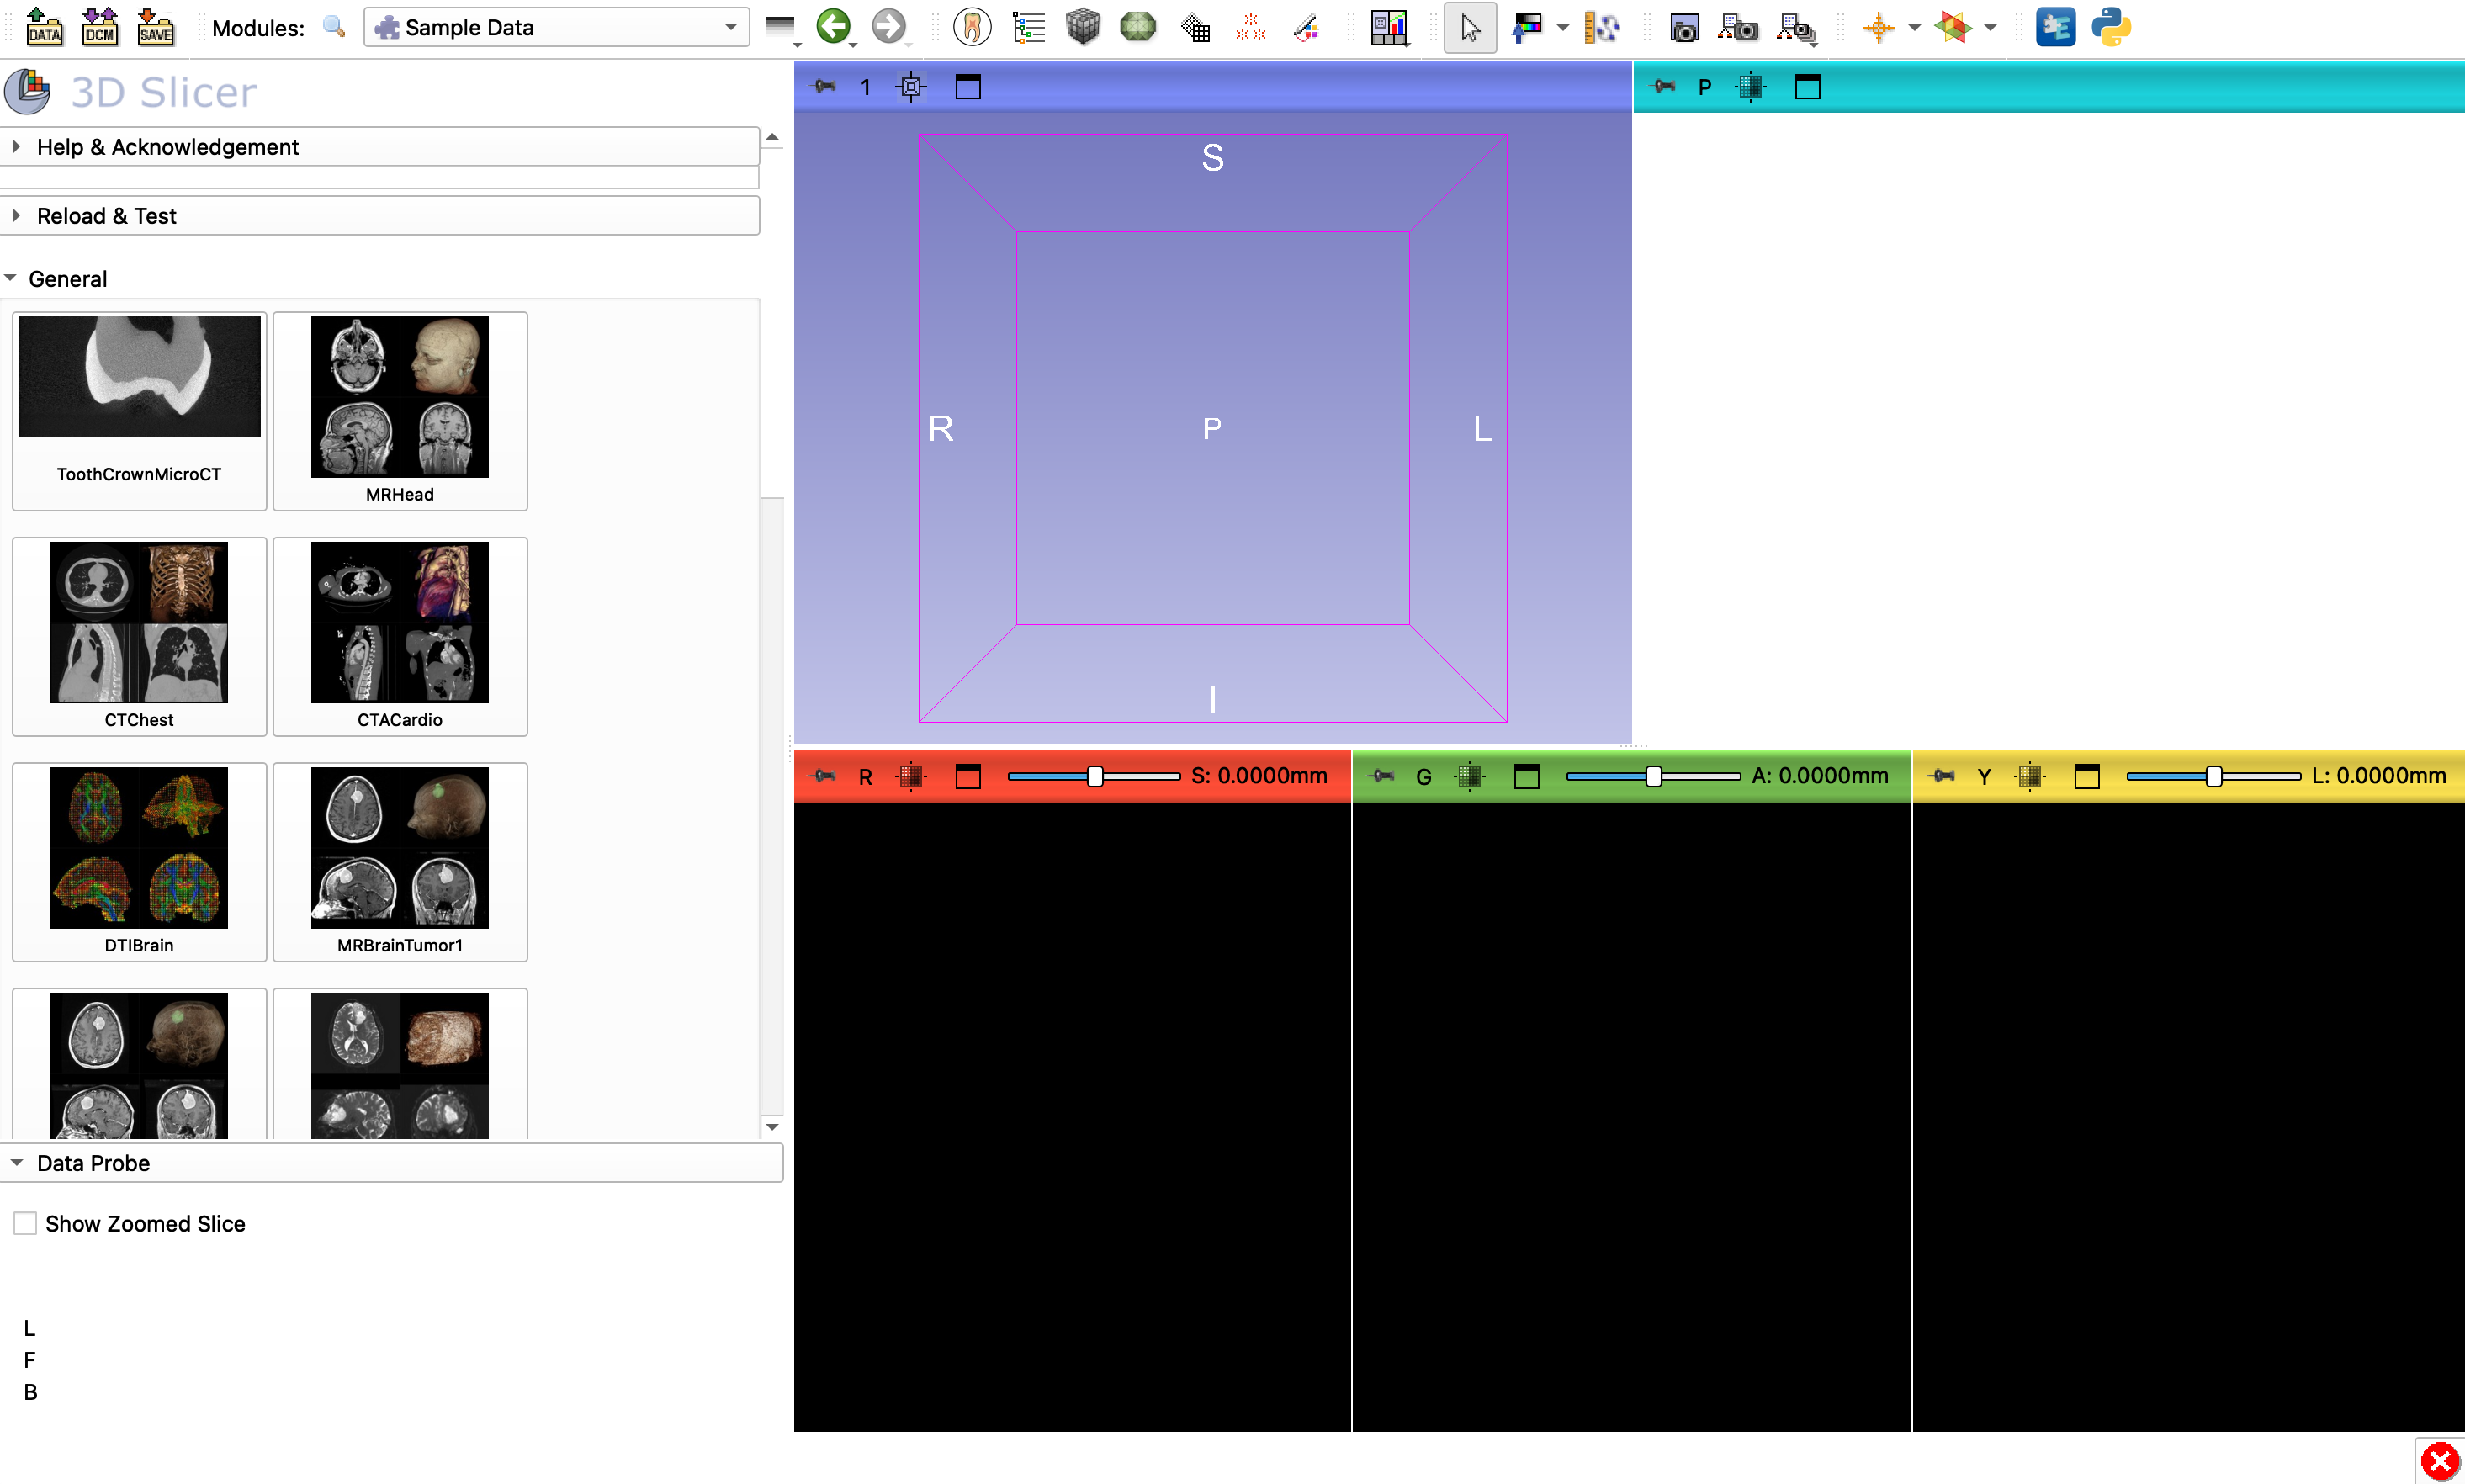
\includegraphics[width=1\textwidth]{img/sampleData.png}
	\caption{Ausschnitt des Moduls SampleData in 3D Slicer mit dem Beispielbild
	für das Starten eines Verfahrens im Tooth Analyser}
	\label{fig:sample_data}
\end{figure}

Ein Testfall der vielen soll hier Beispielhaft genauer betrachtet werden. Hierbei
geht es um den Test der Funktion \texttt{smoothImage()}. Diese Nimmt ein Bild und
führt eine Glättung durch. Um solch eine Funktion zu testen, bedarf es etwas mehr
als ein simplen Unittest, jedoch liefert der fertige Test eine gute Lösung um
den gesamten Umfang der Methode zu Testen. Vergleicht man ein verrauschtes Bild mit
einem geglätteten, dann unterschieden sie sich bis auf die visuelle Darstellung
auch in der Streuung der Pixelwerte. So kann mittels der Standardabweichung kontrolliert
werden, ob das Bild nach einer Filterung eine kleinere Standardabweichung hat
als vor der Filterung. Ist dies der Fall, so kann von einer erfolgreichen
Filterung ausgegangen werden. Zu Beachten ist an dieser Stelle, das eine
Filterung unter Umständen einige Zeit in Anspruch nehmen kann. Es sei gesagt,
dass diese bei einer Testausführung zu berücksichtigen ist. Eine gute Option dem
entgegenzuwirken ist es, das bereits gefilterte Bild mit in den Testdaten zur
Verfügung zu stellen. Die konkrete Implementierung eines solchen Tests liefert der
Quellcode \ref{lst:test_smooth_image}.

\begin{lstlisting}[
    language={python},
    caption={Implementierung eines Tests zum überprüfen einer Funktion},
    label={lst:test_smooth_image}]
def testSmoothImage(self):
    from ToothAnalyserLib.AnatomicalSegmentation.Segmentation import smoothImage
   
    data = self.getSampleDataAsITK()
    dataFiltered = smoothImage(data)
    dataStdDev = np.std(sitk.GetArrayFromImage(data))
    dataFilteredStdDev = np.std(sitk.GetArrayFromImage(dataFiltered))
    self.assertTrue(dataFilteredStdDev < dataStdDev)
    self.delayDisplay("Test 1 passed")
\end{lstlisting}

Im ersten Schritt wird ein Beispielbild geladen und in ein \ac{ITK} Format umgewandelt.
Anschließend folgt die Glättung des Bildes. Ist diese Glättung fertig, so können
die Streuungen der beiden Bilder verglichen werden.

Abschließend lässt sich über die Softwaretests sagen, dass einige Testfälle abgedeckt
wurden. Jedoch wurden nicht alle Methoden und Funktionen getestet. Viele bilden eine
sehr konkrete Lösung, die nicht einfach zu testen ist und deshalb einiges an
Entwicklungszeit beanspruchen. Gerade die Funktionen der Pipeline. Aus diesem
Grund konzentriert sich diese Arbeit nicht auf eine 100 prozentige Testabdeckung,
sondern soll noch weitere Metriken bieten. Eine ebenso gute Aussage lässt sich
anhand der Laufzeit des Moduls treffen. Hierzu wurde die Performance des Tooth Analyser
genauer unter die Lupe genommen und in verschiedenen Szenarien gemessen.

\pagebreak
% ---------------------------------------------------------------------------------------

\section{Performance}
Die Performance des Systems war nie ein wichtiges Kriterium und stand deshalb zu
keiner Zeit im Fokus dieser Arbeit. Dennoch ergaben sich interessante Ergebnisse,
die hier kurz erläutert werden sollen. Unter der Performance versteht dieses Kapitel
das konkrete Laufzeitverhalten der Anwendung also jene Zeit die zwischen Start und
Ende vergeht. Grundsätzlich lässt sich dazu sagen, dass die Laufzeit bei der Bearbeitung
von \ac{3D}-Mikro-\ac{CT}-Aufnahmen sehr stark vom Typ des Bildes abhängt. So
kommt es beispielsweise darauf an, wie groß das Bild ist, oder ob es bereits
eine Filterung erfahren hat. Bei der Verarbeitung der Mikro-\ac{CT}-Bilder aus
dem Klinikum für Zahnerhaltung wurde eine konkrete Messung durchgeführt, die hier
in Abbildung \ref{fig:laufzeit} gezeigt wird.

\textbf{Vorbedingungen:}
\begin{itemize}
	\item 16 bit sigend integer

	\item Type .ISQ

	\item Mit Filterung

	\item Mit Berechnung der medial Flächen
\end{itemize}

\begin{figure}[h]
	\centering
	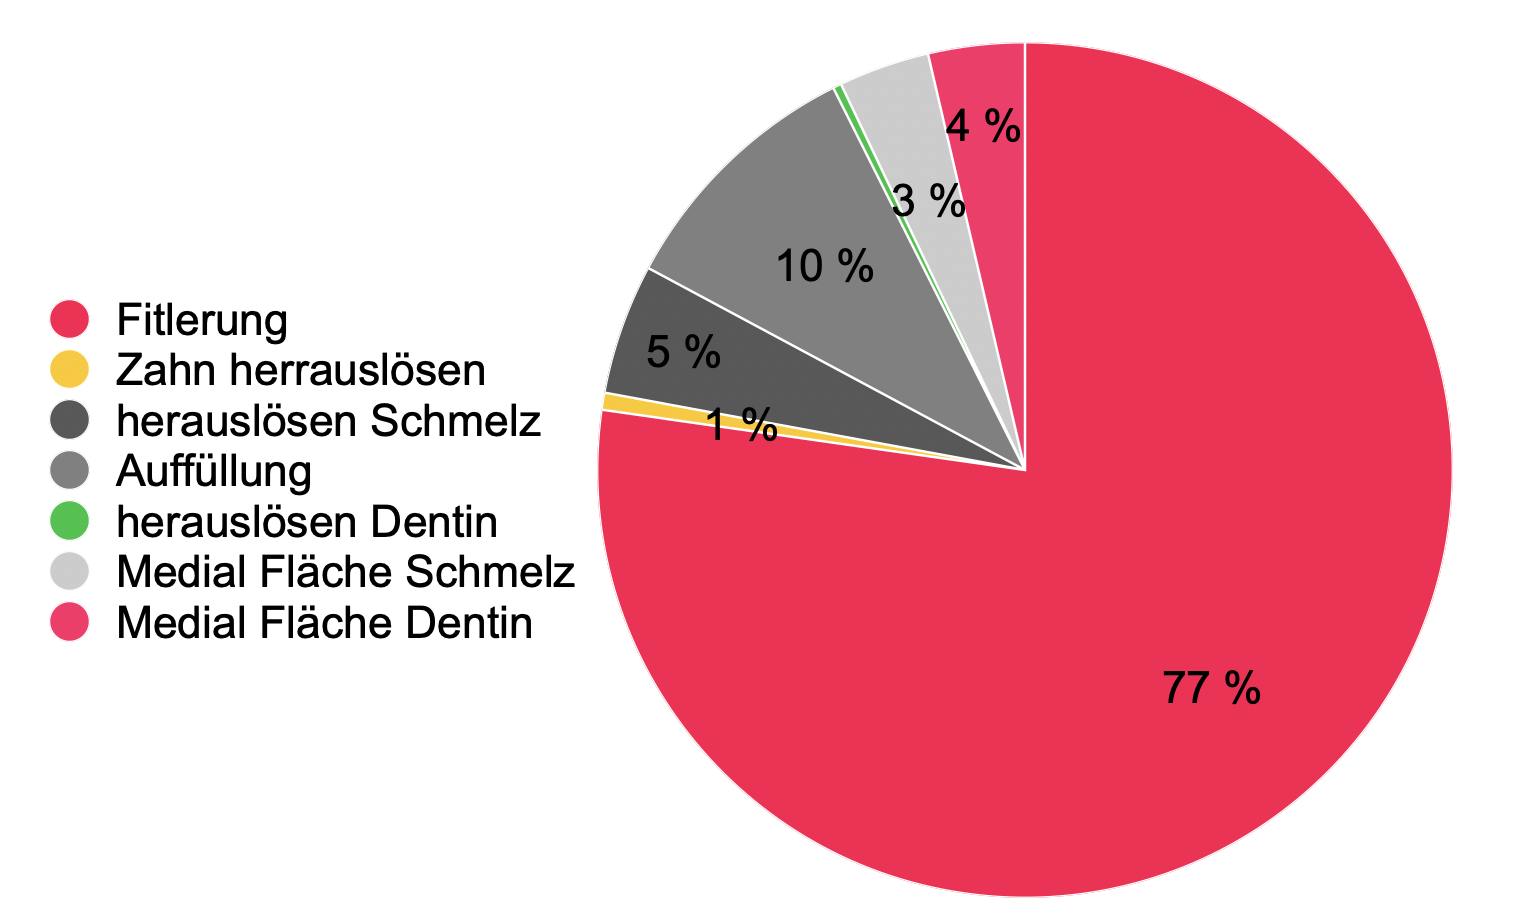
\includegraphics[width=0.8\textwidth]{img/laufzeit_diagramm.png}
	\caption{Verteilung der Laufzeit über den gesamten Bearbeitungszeitraum. 100\%
	entsprechen 16:27 Minuten}
	\label{fig:laufzeit}
\end{figure}

Zu sehen ist, dass unter diesen Bedingungen die Bearbeitung eines einzelnen Bildes
ca. 17 Minuten beansprucht. Dabei fallen über dreiviertel der Zeit auf die Filterung
zurück. Der Bereich Auffüllung beinhaltet ebenfalls eine Filterung der einzelnen
Segmente, weswegen dieser den zweitgrößten Teil ausmacht. Ein Weiterer
wesentlichen Teil stellen die beiden medialen Flächen dar. Um dieser doch enormen
Laufzeit etwas entgegen zu Wirken wurden zwei Mechanismen implementiert. Das
Verfahren kann einerseits erkennen, ob ein Bild bereits gefiltert wurde und andererseits
die medialen Flächen optional berechnen. So kommt es, dass sich ein \textit{Best
Case} ergibt der grob nur noch ein Viertel der Zeit benötigt. Dieser \textit{Best
Case} tritt ein, wenn ein Bild in den Algorithmus gegeben wird, das bereits
gefiltert wurde und keine medialen Flächen erfordert. Unter Berücksichtigung von
Abbildung \ref{fig:laufzeit} kann dann die Zeit für die Filterung und die medialen
Flächen abgezogen werden. So kommt es, dass das Verfahren nur noch 16 Prozent der
ursprünglichen Zeit benötigt.

Überträgt man das Laufzeitverhalten eines einzelnen Bildes auf die Bearbeitung der
Bilder in einem Batch-Prozess so lässt sich die Laufzeit mit der Anzahl der zu bearbeitenden
Bilder steigend linear ausdrücken. Das Diagramm aus \ref{fig:laufzeit_batch}
zeigt dies.

\begin{figure}[h]
	\centering
	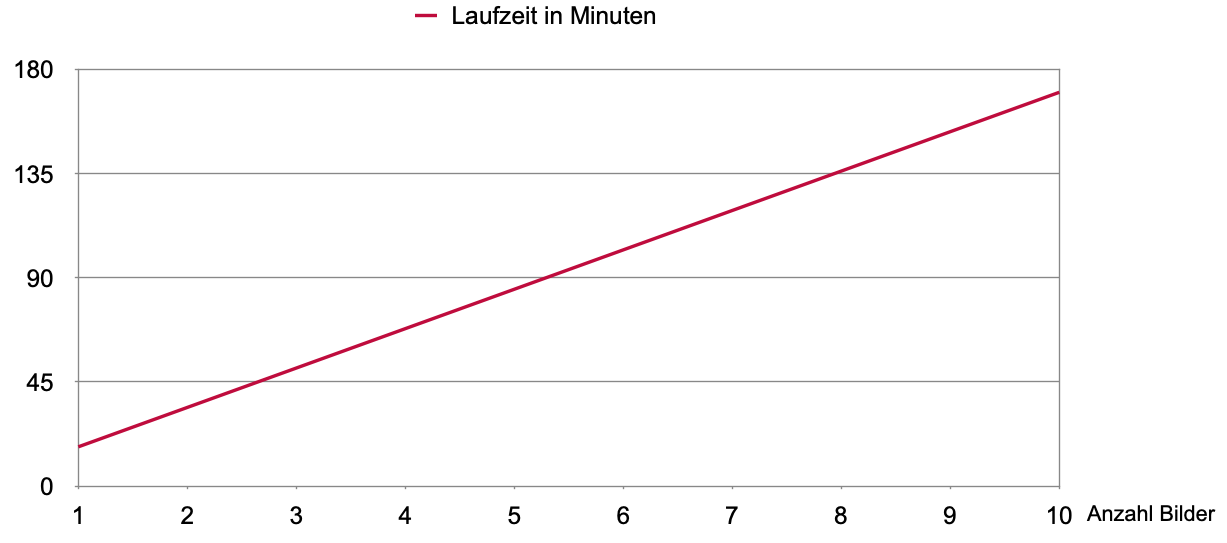
\includegraphics[width=1\textwidth]{img/runtimeBatch.png}
	\caption{Konstruktion des Laufzeitverhaltens bei einer Bearbeitung mehrere
	Bilder}
	\label{fig:laufzeit_batch}
\end{figure}

Wie zu sehen ist, ist die Laufzeit eines Batch Prozesses maßgeblich davon
geprägt, wie lange ein einzelnes Bild benötigt. Dies entspricht dem Y-Achsenabschnitt
im Diagramm \ref{fig:laufzeit_batch}. Ist die Zeit eines einzelnen Bildes bekannt,
so lässt sich gut prognostizieren, wie lange eine Verarbeitung von $n$ vielen Bildern
dauert. Wie bereits angedeutet, hängt die Zeit eines einzelnen Bilds von vielen Faktoren
ab. Nimmt man den Fall aus Abbildung \ref{fig:laufzeit}, würde die Bearbeitung von
zehn Bilder etwa 170 Minuten beanspruchen. Dies entspricht zwei Stunden und 50
Minuten.
% ---------------------------------------------------------------------------------------

\section{Benutzertests}
\label{sec:benutzertests}Um die entwickelte Software objektiv zu bewerten,
wurden gezielte Benutzertests mit Anwendern durchgeführt. Dabei nahmen drei Zahnärzte
der Poliklinik für Zahnerhaltung und Parodontologie an der Testphase teil, in
der sie den Tooth Analyser in ihren Forschungsalltag integrierten. Über einen Zeitraum
von drei Wochen konnten sie die Software in realen Anwendungsszenarien erproben.

Zusätzlich wurde ein kleiner Stresstest durchgeführt, bei dem 103 \ac{CT}-Aufnahmen
in einem Batch-Prozess mit dem Tooth Analyser verarbeitet wurden. Die Berechnung
erfolgte auf einem leistungsstarken Server der LMU, der über ausreichend Rechenkapazitäten
verfügt. Die durchschnittliche Bearbeitungszeit pro Bild lag hier bei etwa neun
Minuten. Basierend auf der in Abbildung \ref{fig:laufzeit_batch} dargestellten Verteilung
ergab sich eine prognostizierte Gesamtverarbeitungszeit von 15 Stunden und 27 Minuten.
Ein Wert, der in der Praxis gut bestätigt wurde. Besonders erfreulich war, dass sämtliche
Bilder bis zu einem gewissen Grad an Karies erfolgreich anatomisch segmentiert werden
konnten. Die Ergebnisse dieses Batch-Prozesses sind dem Anhang zu entnehmen. Die
Tests in der Klinik zeigten zudem, dass auch die vollständige Segmentierung
ganzer Zähne mit komplexen Wurzeln möglich ist.

Die Ergebnisse der Benutzertests aus der Klinik verdeutlichen, dass der Tooth Analyser
in der Praxis eine wertvolle Unterstützung bietet, und durch die Segmentierung
ganzer Zähnen den Anwendungskreis noch weiter spannt. Um ein besseres Verständnis
für die realen Einsatzmöglichkeiten der Software zu gewinnen, werden im
folgenden Kapitel verschiedene Anwendungsszenarien vorgestellt.
% ---------------------------------------------------------------------------------------

\section{Anwendungsszenarien}
In erster Linie bietet der Tooth Analyser eine Visualisierungshilfe, die für Ärzte
unterstützend wirken soll. Wie auch von Slicer empfohlen wird dieses Modul von
den Ärzten rein zur Forschung eingesetzt. Mit dem Tooth Analyser lässt sich mittels
einer Mikro-\ac{CT}-Aufnahme ein \ac{3D}-Modell des Zahnes erstellen. Man
spricht hier von einer Rekonstruktion des Zahnes. Durch die Segmentierung erlaubt
dieser rekonstruierte Zahn auch eine Segmentbetrachtung von Dentin und Schmelz.
Die Abbildungen \ref{fig:3d_view}, \ref{fig:3d_view_dentin} und \ref{fig:3d_view_schmelz}
zeigt diese Rekonstruktion genauer.

\begin{figure}[h]
	\centering
	\begin{minipage}[b]{0.32\textwidth}
		\centering
		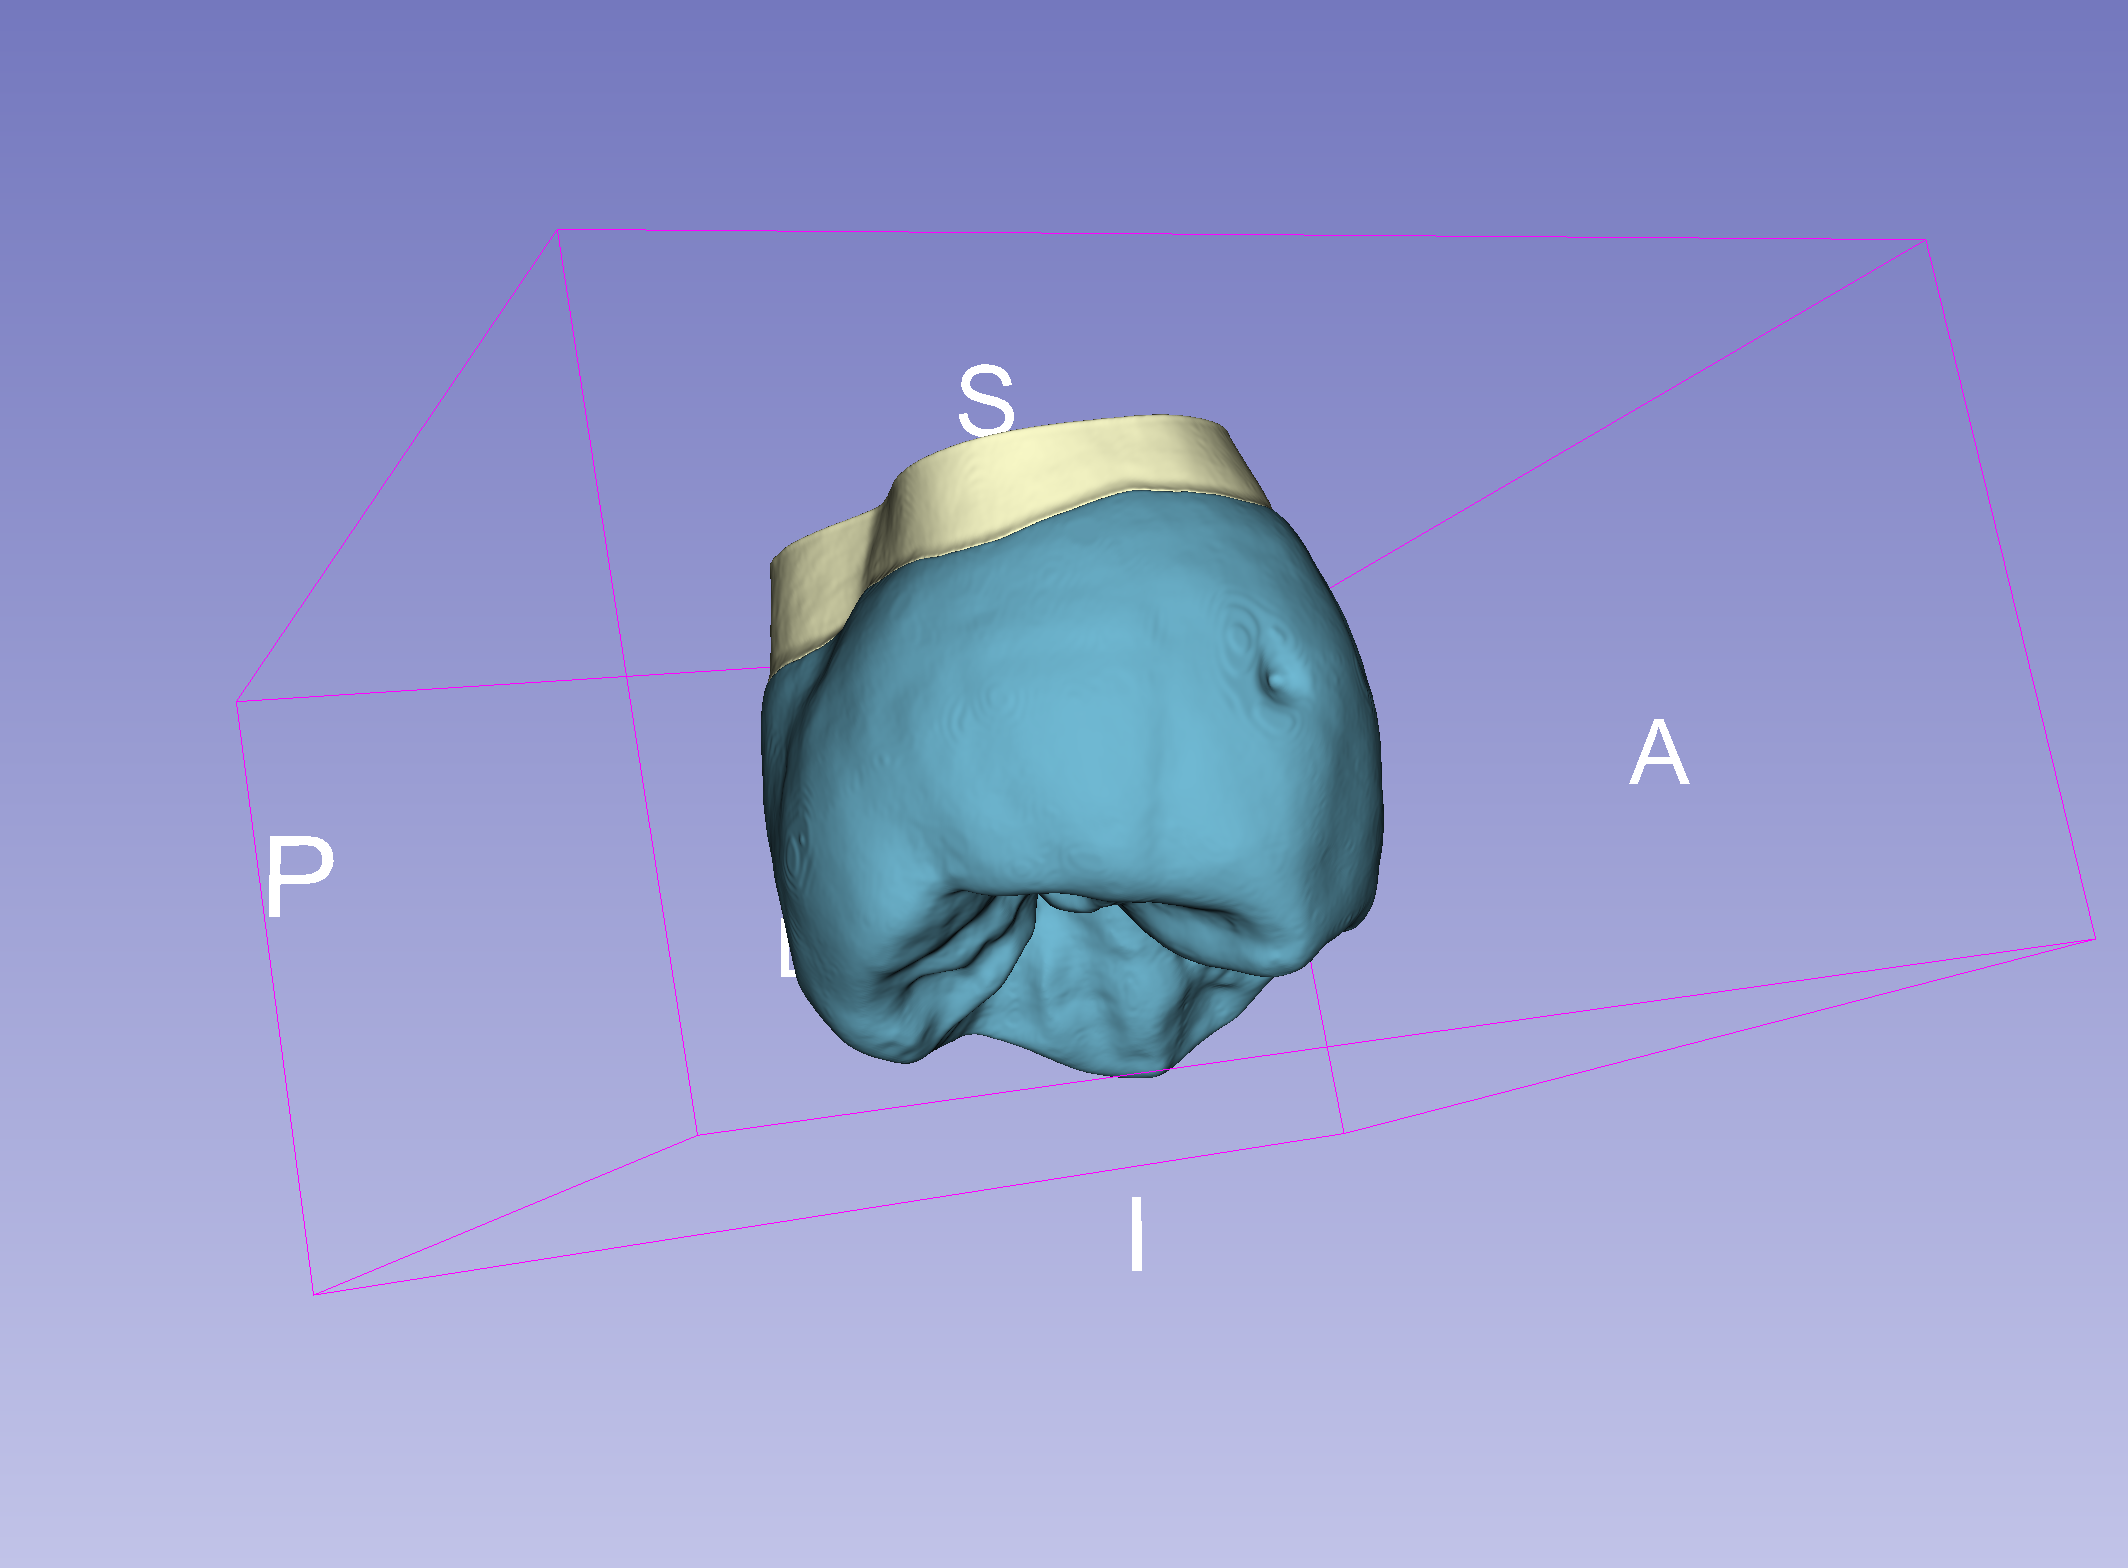
\includegraphics[width=\textwidth]{img/3dView.png}
		\caption{Rekonstruktion eines Zahns aus einer CT-Aufnahme}
		\label{fig:3d_view}
	\end{minipage}
	\hfill
	\begin{minipage}[b]{0.32\textwidth}
		\centering
		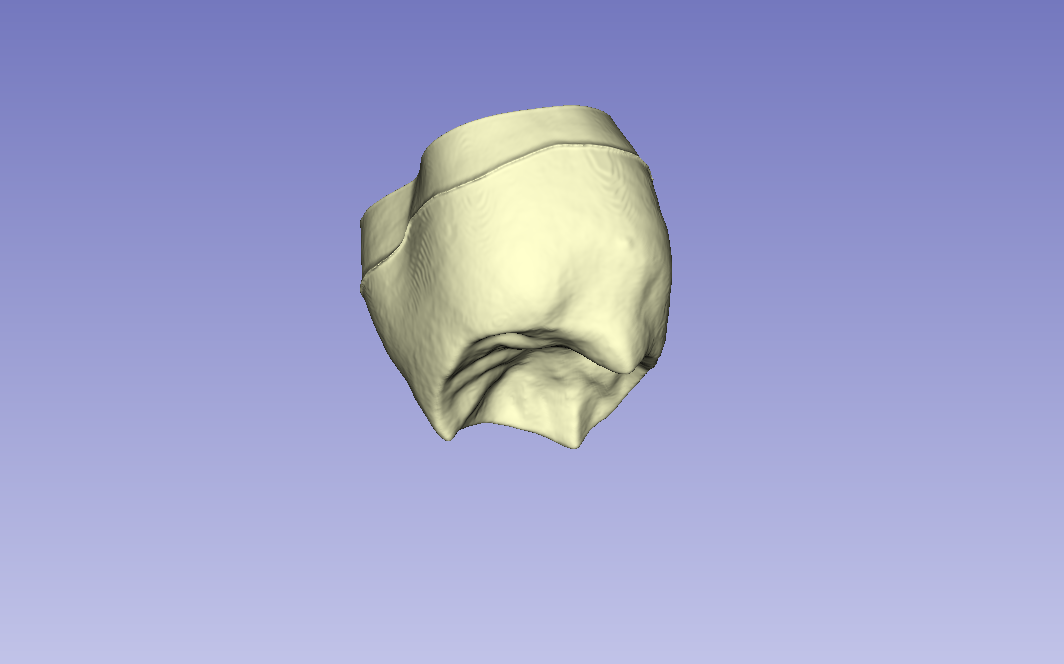
\includegraphics[width=\textwidth]{img/3dViewDentin.png}
		\caption{Dentinsegment eines rekonstruierten Zahns}
		\label{fig:3d_view_dentin}
	\end{minipage}
	\hfill
	\begin{minipage}[b]{0.32\textwidth}
		\centering
		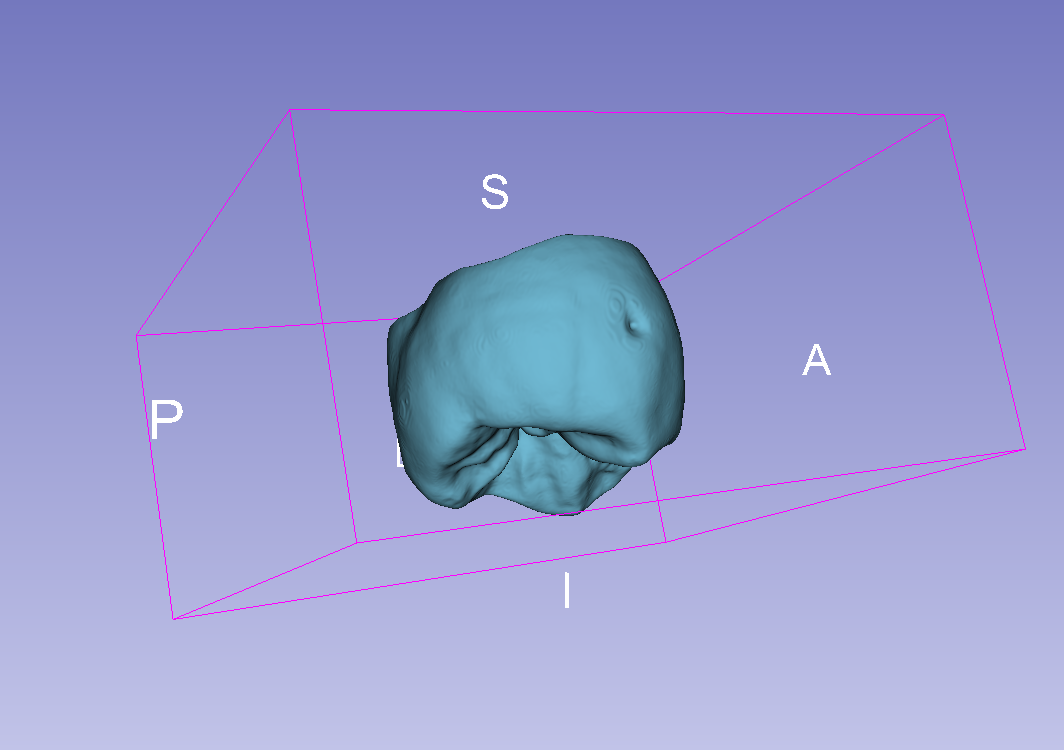
\includegraphics[width=\textwidth]{img/3dViewEnamel.png}
		\caption{Schmelzsegment eines rekonstruierten Zahns}
		\label{fig:3d_view_schmelz}
	\end{minipage}
\end{figure}

Das Betrachten der einzelnen Segmente wie sie in Abbildung
\ref{fig:3d_view_dentin} gezeigt wird, erfolgt nicht in der Erweiterung Tooth Analyser.
Hierzu wird auf das Modul \textit{Data} verwiesen, das eine hierarchische
Darstellung aller Daten in der Szene liefert. Über die Sichtbarkeitseinstellungen
der einzelnen Datenelemente können dann die Segmente sichtbar oder unsichtbar geschaltet
werden.

Einen weiteren Fall, indem die Anwendung unterstützen kann, ist die Klassifizierung
von Karies. Die Abbildung \ref{fig:classification} zeigt diesen Fall. Hierfür sind
die medialen Flächen der einzelnen Segmente nötig. Diese sind im Bild als rote
und grüne Linie sichtbar, verteilen sich aber über das ganze \ac{3D}-Bild, was daraus
eine Fläche macht. Legt man nun diese Flächen über das originale Bild, so lässt sich
mittels dieser Linie der Karies auf einem \ac{CT} gut klassifizieren. Diese besagten
Linien bilden dann die Grenzen. Ragt der Karies über diese mediale Fläche hinaus
hat er bereits einen sehr ausgeprägten Zustand und wird anders eingeordnet als
ein Karies, der die mediale Fläche noch nicht überschritten hat.

\begin{figure}[h]
	\centering
	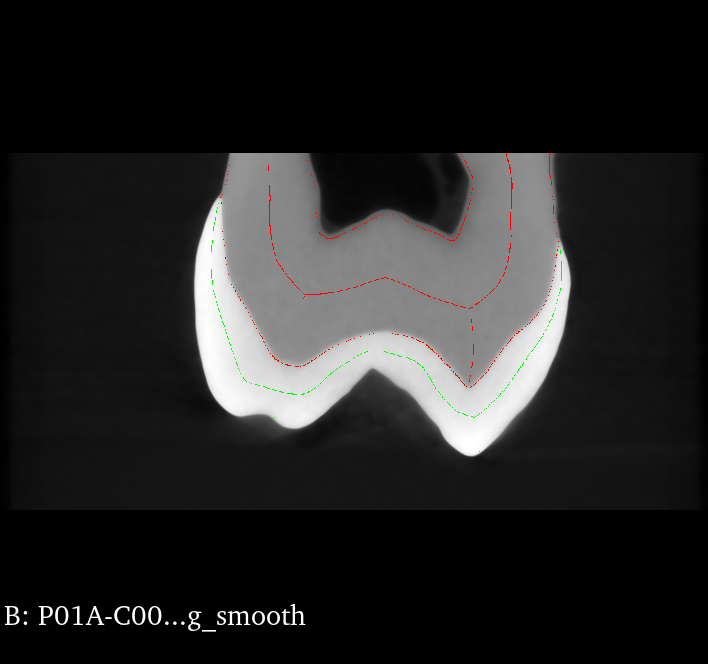
\includegraphics[width=0.4 \textwidth]{img/classification.png}
	\caption{Klassifizierung von Karies mittels der medialen Flächen}
	\label{fig:classification}
\end{figure}

Die konkreten Anwendungsfälle zeigen, dass der Tooth Analyser durchaus Anwendung
im Forschungsalltag der Klinik finden. Dennoch traten während der Nutzung auch
einige Einschränkungen auf, die die Einsatzmöglichkeiten des Tooth Analyser begrenzen.
% ---------------------------------------------------------------------------------------

\section{Limitierungen}
\label{sec:limitierungen} Dieses Kapitel soll alle Punkte transparent aufdecken,
die im Modul Tooth Analyser noch Probleme machen, oder gar nicht erst umgesetzt wurden.
Der limitierende Faktor in der Erweiterung ist das eingeschränkte Format der
Bilder. Es können innerhalb dieser Erweiterung nur Bilder verarbeitet werden,
die das Format \ac{16Int} haben. Führt man dennoch die Segmentierung mit einem
anderen Format durch (z.B. \ac{8UInt}), so stellt man fest, dass der Algorithmus
zwar ein Ergebnis generiert, dieses aber nicht verwendbar ist. Die Abbildung
\ref{fig:3d_error} zeigt ein solches falsche Ergebnis. Zu sehen ist ein \ac{3D}-Modell,
das nur aus einem Segment besteht. In diesem Fall wurde der gesamte Zahn mit
Pulpa als Dentin markiert.

\begin{figure}[h]
	\centering
	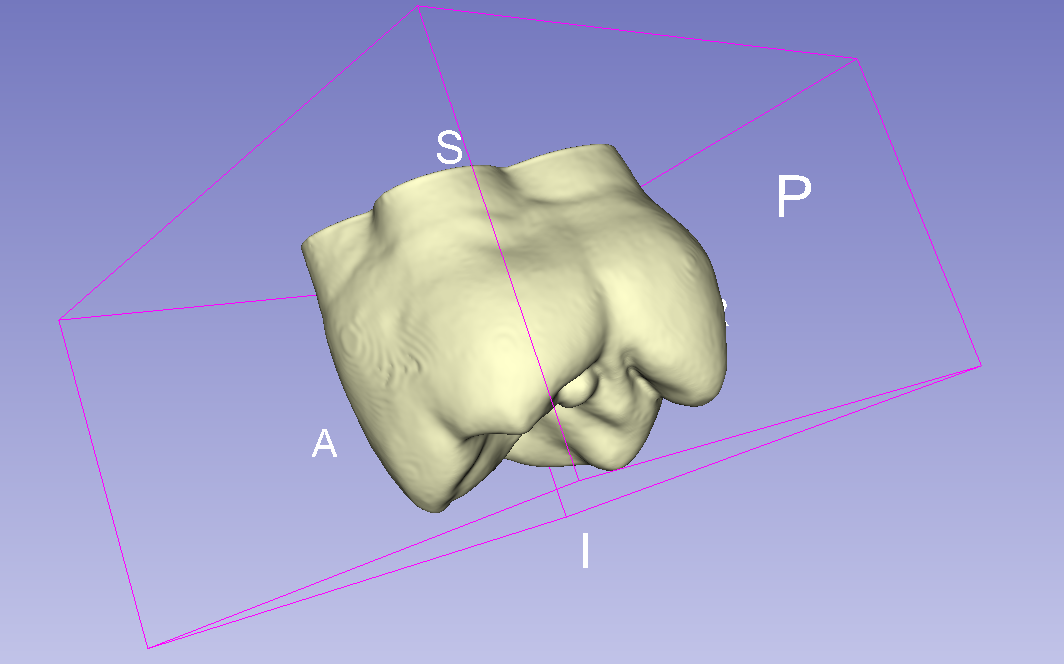
\includegraphics[width=0.5\textwidth]{img/3d_view_error.png}
	\caption{Fehlerhafte Segmentierung einer CT-Aufnahme im Format 8UInt}
	\label{fig:3d_error}
\end{figure}

Durch diese Limitierung ergibt sich eine weitere. Zu Beginn in der Analysephase
des Projektes, war eine Vorverarbeitung der Bilder vorgesehen, dass die
Komprimierung eines Bildes vornimmt und so die Bilder deutlich handlicher macht.
Das Verfahren hierzu wurde in Kapitel \ref{subsec:datensätze} erläutert. Da
dieses Verfahren allerdings einen Formatwechsel von \ac{16Int} nach \ac{8UInt}
bewirkt und diese Bilder nicht richtig segmentiert werden können, scheidet die Vorverarbeitung
von Bildern vorerst aus.

Eine weitere Limitierung liegt im Batch-Modus. Dieser steht laut der Struktur in
Kapitel \ref{sec:struktur_der_software} nicht nur für die ganze
Verarbeitungspipeline zur Verfügung, sondern auch für die einzelnen Schritte dieser
Pipeline. Da eine konkret implementierte Vorverarbeitung ohnehin vorerst
ausscheidet, wurde der Batch-Prozess nur für die reine anatomische Segmentierung
implementiert.

Zuletzt sei noch auf eine Limitierung hingewiesen, die der Erweiterbarkeit des
Moduls dient. Soll die Erweiterung um zusätzliche Funktionen erweiter werden,
dann sind kleine Änderungen in einer bestehenden Klasse notwendig. Konkret geht es
hier um die Klasse \texttt{ToothAnalyserWidget}. Hier muss je nach Ausprägung der
\ac{UI} der neuen Funktion, Methoden hinzugefügt werden.
% ---------------------------------------------------------------------------------------
	\chapter{Diskussion}
\label{chap:diskussion} Am Ende dieser Arbeit lohnt es sich, erneut einen Blick
auf die in Kapitel \ref{sec:ziel_der_arbeit} formulierte Forschungsfrage zu
werfen und noch einige Aspekte hinzuzufügen:

\begin{center}
	\textit{Wie kann eine benutzerfreundliche Schnittstelle innerhalb von 3D
	Slicer entwickelt werden, die nicht nur das Verfahren der anatomischen Segmentierung
	effizient integriert und den Zugang für Anwender vereinfacht, sondern auch
	eine strukturierte und flexible Umgebung zur Verarbeitung von Mikro-\ac{CT}-Aufnahmen
	bietet?}
\end{center}

Die Ergebnisse dieser Arbeit zeigen, dass die Integration der anatomischen
Segmentierung erfolgreich in das Ökosystem von 3D Slicer eingebunden werden
konnte. Das zuvor komplexe und manuell aufwendige Verfahren wurde durch die entwickelte
Benutzeroberfläche erheblich vereinfacht. Anstelle einer umständlichen Terminal-Nutzung
kann die Segmentierung nun mit wenigen Klicks gestartet werden, was insbesondere
die praktische Anwendung in der Zahnmedizin erheblich erleichtert.

Ein zentraler Aspekt der Forschungsfrage betraf die Effizienz der Integration.
Hier konnte gezeigt werden, dass das entwickelte Modul zuverlässige Ergebnisse liefert,
ohne dabei die Qualität der anatomischen Segmentierung zu beeinträchtigen. Mit dem
Tooth Analyser entstand somit eine durchdachte Struktur für die Verarbeitung von
Mikro-\ac{CT}-Aufnahmen, die einen bedeutenden Fortschritt für die zahnmedizinische
Forschung darstellt. Der Luxus einer interaktiven Schnittstelle ist dabei nur
die Spitze des Eisbergs. Die wohl wichtigste Erkenntnis, die diese vorliegende
Arbeit liefert, ist das zugrunde liegende Modell, mit dem eine effiziente und
interaktive Bearbeitung von Mikro-CT-Aufnahmen möglich ist. Diese Struktur erwies
sich als äußerst effektiv im klinischen Forschungsalltag. Insbesondere konnte
beobachtet werden, dass es neben der Ausführung einer ganzen Bearbeitungspipeline
auch sinnvoll ist einzelne Schritte in der Pipeline isoliert ausführen zu können.
Diese Aspekte betreffen auch den Batch-Prozess, der eine ganze Sammlung an Bilder
auf einmal verarbeiten kann.

Neben der verbesserten Flexibilität wurde auch die Effizienz des Workflows gesteigert.
Eine manuelle Segmentierung eines einzelnen Zahns nimmt durchschnittlich rund 20
Minuten in Anspruch. Durch den Tooth Analyser kann dieser Prozess vollständig automatisiert
im Hintergrund ablaufen, wodurch wertvolle Zeit eingespart wird. Laut Dr. Elias
Walter reduziert sich der aktive Arbeitsaufwand dadurch erheblich, da die Segmentierung
nicht mehr manuell durchgeführt werden muss.

Ein Punkt, der zu Beginn der Entwicklung nicht feststand, war die optionale Generierung
der medialen Flächen sowie die automatische Erkennung bereits gefilterter Bilder.
Beide Funktionen sind das Ergebnis der Laufzeitmessung und tragen zur
Effizienzsteigerung der Anwendung bei. Die optionale Generierung medialer Flächen
ermöglicht es, die Berechnung gezielt an- oder auszuschalten, je nach den
Anforderungen des jeweiligen Anwendungsfalls. Dadurch wird verhindert, dass
unnötige Rechenoperationen ausgeführt werden, wenn diese für die Analyse nicht erforderlich
sind. Die automatische Erkennung bereits gefilterter Bilder sorgt dafür, dass doppelte
Verarbeitungsschritte vermieden werden. Anstatt ein Bild erneut durch die
gesamte Pipeline zu schicken, erkennt das System, ob eine vorherige Filterung
bereits erfolgt ist, und kann das Bild direkt für die nächste Verarbeitungsstufe
nutzen.

Aus den Anforderungen ging auch hervor, dass bei einer mehrfachen Erstellung der
segmentierten Daten aus einem Mikro-\ac{CT}, die Slicer-Szene die alten Daten
immer Überschreiben soll. So wird sichergestellt, dass immer nur die aktuelle
Segmentierung sichtbar ist. Das Ergebnis hat gezeigt, dass dieses Verhalten
durchaus sinnvoll ist. Jedoch ist es hilfreich neben der Segmentierung selbst,
auch noch das originale Mikro-\ac{CT} in der Szene zu halten, sodass der Kontext
sichtbar beliebt.

Auch die Erweiterbarkeit des Systems wurde berücksichtigt. Dank der modularen Architektur
kann das zugrunde liegende Segmentierungsverfahren ohne größere Anpassungen ausgetauscht
oder durch weitere Funktionalitäten ergänzt werden. Dies gewährleistet
langfristige Flexibilität und Anpassungsfähigkeit an zukünftige Entwicklungen. Gleichzeitig
zeigte sich jedoch auch, dass eine große Anzahl an Funktionen im Modul zu einer
Überladung der \ac{UI} führen kann. Um dies in der Zukunft zu vermeiden, kann die
3D Slicer Erweiterung auf mehrere Module aufgeteilt werden, die einen logischen
und inhaltlichen Zusammenhang haben.

Zur objektiven Evaluation wurden Benutzertests mit mehreren Zahnärzten der
Klinik durchgeführt. Über einen Zeitraum von drei Wochen integrierten sie den Tooth
Analyser in ihren Forschungsalltag. Dabei gelang nicht nur die Segmentierung
einzelner Zahnkronen, sondern auch vollständiger Zähne mit komplexen Wurzeln.
Besonders bemerkenswert ist, dass die Software während der gesamten Entwicklung ausschließlich
mit \ac{CT}-Aufnahmen von Zahnkronen getestet wurde. Dennoch konnte sie ohne zusätzliche
Anpassungen auch diese erweiterte Anwendungsform erfolgreich bewältigen. Dies
unterstreicht die Flexibilität des Systems und stellt einen bedeutenden Erfolg
dar. Grundsätzlich lässt sich sagen, dass die Benutzertests für diese Arbeit die
wichtigste Evaluationsgrundlage bilden.

In einem weiteren Test wurde die Skalierbarkeit der Anwendung überprüft. Hierbei
wurden 103 Mikro-\ac{CT}-Aufnahmen in einem Batch-Prozess über einen
leistungsstarken Server der LMU verarbeitet. Die Bearbeitungszeit pro Bild lag bei
etwa neun Minuten, sodass eine Gesamtzeit von etwa 15 Stunden und 27 Minuten
prognostiziert wurde – ein Wert, der sich in der Praxis bestätigte. Entscheidend
war jedoch, dass alle Bilder erfolgreich anatomisch segmentiert werden konnten.

Trotz der vielen positiven Ergebnisse zeigen sich auch einige Einschränkungen.
Die wesentlichen wurden bereits im Kapitel Limitation erwähnt. So kommt es, das
die anatomische Segmentierung speziell für Mikro-\ac{CT}-Aufnahmen im \ac{ISQ}-Format
entwickelt wurde, wodurch bestimmte Parameter und Schwellwerte fest im Code hinterlegt
wurden. Dies schränkt die Flexibilität bei der Nutzung mit anderen Bildformaten
ein. Eine detaillierte Analyse der Segmentierungsergebnisse zeigte, dass das
Problem im Bereich der Auffüllung liegt. Zu Beginn der Segmentierung werden die Zahnbestandteile,
einschließlich der Pulpa, korrekt erkannt. Während der anschließenden Auffüllung
des Schmelzsegments kommt es jedoch zu einer fehlerhaften Überschreibung bereits
richtig segmentierter Strukturen. Diese wohl größte Limitierung des Tooth Analyser
führt auf eine weitere, welche die Vorverarbeitung von Bilder betrifft.

Die Implementierung einer Vorverarbeitung der Bilder konnte bislang nicht
umgesetzt werden. Zwar ist diese Funktionalität bereits konzeptionell vorgesehen,
jedoch bedarf es noch weiterer Arbeit, um eine vollumfängliche Implementierung zu
ermöglichen. Der Grund hierfür ist, dass innerhalb der Vorverarbeitung eine Komprimierung
der Bilder geplant war. Diese Komprimierung zieht jedoch auch einen
Formatwechsel von \ac{16Int} auf \ac{8UInt} nach sich. Da diese Bilder ohnehin nicht
bearbeitet werden können, wurde hierfür keine Implementierung bereitgestellt. Zur
Vorverarbeitung der Bilder kann grundsätzlich noch eine andere Überlegung angestellt
werden. Die anatomische Segmentierung enthält eine umfangreiche Filterung zur
Rauschreduktion. Laut der Visualisierungspipeline nach \citet[S.~50]{handels2000},
gehört dieser Schritt auch zu einer Vorverarbeitung. Eine gute Idee ist es also,
die Filterung der anatomischen Segmentierung aus dem eigentlichen Verfahren herauszuziehen
und im Bereich der Vorverarbeitung bereitzustellen. Dies ermöglicht auch ein
Filter der Bilder, unabhängig von einer anschließenden Segmentierung.

Eine Gute Idee zeigt sich auch im Bereich der Analysen. Diese stehen aktuell als
eigenes Verfahren bereit. Wie bereits beschrieben, könnten diese auch im Bereich
der Nachverarbeitung einen Platz finden. Anstelle der Analysen als Verfahren,
könnte dann eine andere Art der Segmentierung implementiert werden.

Zusammenfassend lässt sich sagen, dass die in dieser Arbeit entwickelte Lösung die
Forschungsfrage in wesentlichen Punkten beantworten konnte: Die Segmentierung
wurde effizient in 3D Slicer integriert, die Benutzerfreundlichkeit erheblich verbessert
und die Softwarearchitektur flexibel gestaltet. Darüber hinaus wurde ein
strukturiertes Modell für die effiziente und interaktive Verarbeitung von Mikro-\ac{CT}-Aufnahmen
entwickelt. Nichtsdestotrotz ist das System noch nicht in seinem finalen
Entwicklungsstadium. Insbesondere weitere Benutzertests und Anpassungen der Parameter
innerhalb der Segmentierung könnten zu einer noch höheren Präzision und Benutzerfreundlichkeit
beitragen. Auch die in Kapitel \ref{sec:relevanz_der_arbeit} diskutierte
Relevanz der Arbeit zeigt, dass der Tooth Analyser zwar bereits einen großen Fortschritt
darstellt, jedoch noch Optimierungen erforderlich sind, um eine langfristig etablierte
und klinisch einsetzbare Lösung zu erreichen.
% ---------------------------------------------------------------------------------------
	\chapter{Ausblick}
\label{chap:schlussfolgerung} Der Tooth Analyser bietet mit dem aktuellen Stand bereits
einen großen Mehrwert für die Ärzte in der Klinik für Zahnerhaltung. So lässt
sich sagen, dass diese vorliegende Arbeit durchaus von Erfolg gekrönt ist. Es
wird aber auch klar, dass noch viel Potenzial im Tooth Analyser steckt. Das
meiste Potenzial ist hierbei in den Limitierungen zu finden. Eine hervorragende Ergänzung
dieser Arbeit würde eine Vorverarbeitung der Bilder bieten. Es soll also in
Zukunft möglich sein, die \ac{CT}-Aufnahmen in einer Vorverarbeitung zu
komprimieren und sie dann mittels eines Verfahren zu bearbeiten. Hierbei muss sich
die Vorverarbeitung nicht auf die Komprimierung beschränken, wie die Diskussion
gezeigt hat. Dies schließt auch eine Verarbeitung aller Formate ein. Ein schöner
Nebeneffekt dieser Ergänzung ist, dass durch eine Komprimierung der Bilder die Laufzeit
sinkt. Der verlorene Detailgrad dieser Komprimierung ist dabei nicht störend. Somit
lässt sich sagen, dass durch das Akzeptieren unterschiedlicher Formate der
größte Mehrwert für den Tooth Analyser gewonnen werden kann. Des Weiteren lässt der
Bereich Analysen im Tooth Analyser noch viel Spielraum. Hier gibt es diverse
Möglichkeiten, das Modul noch mit weiteren Funktionen zu bestücken. Eine gute
Idee lieferte hier die Rückmeldung aus den Benutzertests. Diese ergaben, dass
eine Integration des Python-Pakets \textit{radiomics} den Tooth Analyser gut ergänzen
würde. Mit diesem Paket lassen sich Radiomics-Merkmale aus Bilder Extrahieren
und isoliert analysieren. Den letzten Ausblick, der hier gegeben werden soll, bezieht
sich wieder auf das Verfahren der anatomischen Segmentierung. In der aktuellen
Version nimmt das Verfahren nur eine Aufteilung in Schmelz und Dentin vor. Der Teil
der Pulpa wird dem Hintergrund zugeordnet und nicht betrachtet. Die zusätzliche
Segmentierung der Pulpa würde die Arbeit ebenfalls hervorragend ergänzen. Jedoch
sei auch gesagt, das dies die wohl herausforderndste Aufgabe ist. Die Pulpa hebt
sich nur sehr leicht aus dem Hintergrund hervor und ist demnach schwer zu segmentieren.

Ordnet man die hier genannten Punkte nach ihrer Wichtigkeit ein, so lässt sich
sagen, das durch das Erweitern des Moduls auf mehrere Bildformate der größte Mehrwert
für den Tooth Analyser gewonnen werden kann. Dies würde weitere Funktionalität
nach sich ziehen. Jedoch sei auch gesagt, dass die übrigen Punkte ebenfalls
einen großen Mehrwert für den Tooth Analyser und damit für die gesamte
Zahnmedizin bietet.
% ---------------------------------------------------------------------------------------

	% --------------------------------------------------
	% Bibliographie
	% --------------------------------------------------
	\renewcommand{\bibfont}{\footnotesize}
	\printbibliography
	[title={Literaturverzeichnis}, heading=bibintoc]

	% --------------------------------------------------
	% Anhang
	% --------------------------------------------------
	\appendix
	\chapter{Anhang}
\label{chap:anhang} test
	\AuthorDeclaration % Selbständigkeitserklärung

	% --------------------------------------------------
	% Index
	% --------------------------------------------------
	{\setkomafont{section}{\Huge} % temporarily set chapter font
	\printindex }
\end{document}